\documentclass{article}
\usepackage[utf8]{inputenc}
\usepackage{polski}
\usepackage[polish]{babel}
\usepackage{graphicx}
\usepackage{amsmath}
\usepackage{listings}
\usepackage{hyperref}
\usepackage{float}

\title{POP - Projekt - Sprawozdanie końcowe}
\author{Adam Czupryński \and Szymon Makuch}

\begin{document}
\maketitle

\section{Temat projektu}
Ewolucja różnicowa z modyfikacją wdrażającą nieszablonowy model zastępczy (surrogate model) w celu optymalizacji procesu selekcji osobników z populacji do ewaluacji funkcji celu.

\section{Opis problemu}
Ewolucja różnicowa (DE) jest skutecznym algorytmem optymalizacji globalnej, jednak jej główną wadą jest duża liczba wymaganych ewaluacji funkcji celu. W przypadku gdy obliczenie wartości funkcji celu jest czasochłonne lub kosztowne, może to znacząco ograniczać praktyczne zastosowanie algorytmu. Rozwiązaniem tego problemu może być zastosowanie modelu zastępczego (surrogate model), który aproksymuje wartość funkcji celu na podstawie wcześniej obliczonych punktów.

\section{Implementacja}
Projekt został zaimplementowany w języku Python. Główny algorytm ewolucji różnicowej znajduje się w pliku differential\_evolution.py, natomiast jego zmodyfikowana wersja wykorzystująca model zastępczy w surrogate\_de.py. Funkcje testowe z benchmarku CEC oraz pomocnicze funkcje do przeprowadzania eksperymentów znajdują się odpowiednio w plikach functions.py oraz experiments.py. Skrypty parameter\_tuning.py oraz tree\_parameters\_tuning.py służą do wyznaczenia optymalnych parametrów algorytmów ewolucji różnicowej oraz modelu zastępczego.

Wykresy zostały wygenerowane przy użyciu biblioteki pyplot. Informacje dotyczące sposobu odczytywania informacji z wykresu pudełkowego można znaleźć na stronie: \url{https://matplotlib.org/stable/api/_as_gen/matplotlib.pyplot.boxplot.html}.

\section{Ewolucja różnicowa}
Zaimplementowaliśmy algorytm ewolucji różnicowej z dwoma kryteriami stopu: maksymalną liczbą generacji oraz brakiem poprawy najlepszego osobnika przez określoną liczbę generacji.
Maksymalna liczba ewaluacji jest więc równa iloczynowi maksymalnej liczby generacji i wielkości populacji. Zawsze jednak istnieje szansa na zatrzymanie algorytmu przez kryterium stopu stagnacji. Polego ono na sprawdzeniu czy przez określoną liczbę iteracji nie nastąpiła poprawa najlepszego osobnika. Jeżeli taka poprawa nie nastąpiła, algorytm kończy działanie.

Do testowania algorytmu zostały użyte następujące zakresy parametrów:

\begin{enumerate}
    \item CR - prawdopodobieństwo krzyżowania. Wartość parametru CR jest definicyjnie narzucona i musi znajdować się w przedziale od 0 do 1.
    \item F - współczynnik mutacji.
    \item Population size - wielkość populacji - dodatnia liczba całkowita.
    \item Max generations - maksymalna liczba generacji - dodatnia liczba całkowita.
    \item Stagnation - liczba generacji bez poprawy najlepszego osobnika - dodatnia liczba całkowita.
\end{enumerate}

\subsection{Wyznaczanie parametrów ewolucji}

Badanie zaczęliśmy od wyznaczania optymalnych parametrów ewolucji różnicowej. W tym celu przeprowadziliśmy eksperymenty dla funkcji Shifted Rotated Griewank z benchmarku CEC o 2 wymiarach. Wyznaczanie optymalnych parametrów algorytmu ewolucji różnicowej rozpoczęliśmy od wybrania domyślnych wartości wszystkich testowanych parametrów, które wydawały nam się sensowne. Dla tych wartości rozpoczęliśmy testowanie pojedynczych parametrów aby uzyskać przedziały wartości, które dają najlepsze wyniki. Dla najlepszych znalezionych przedziałów wartości przeprowadzaliśmyk kolejne testy, które ostatecznie pozwoliły nam na wybranie optymalnych wartości parametrów do dalszych testów. Procent sukcesu, na podstawie którego sprawdzaliśmy jakość parametrów był uśredniany po 50 iteracjach.

\begin{figure}[H]
    \centering
    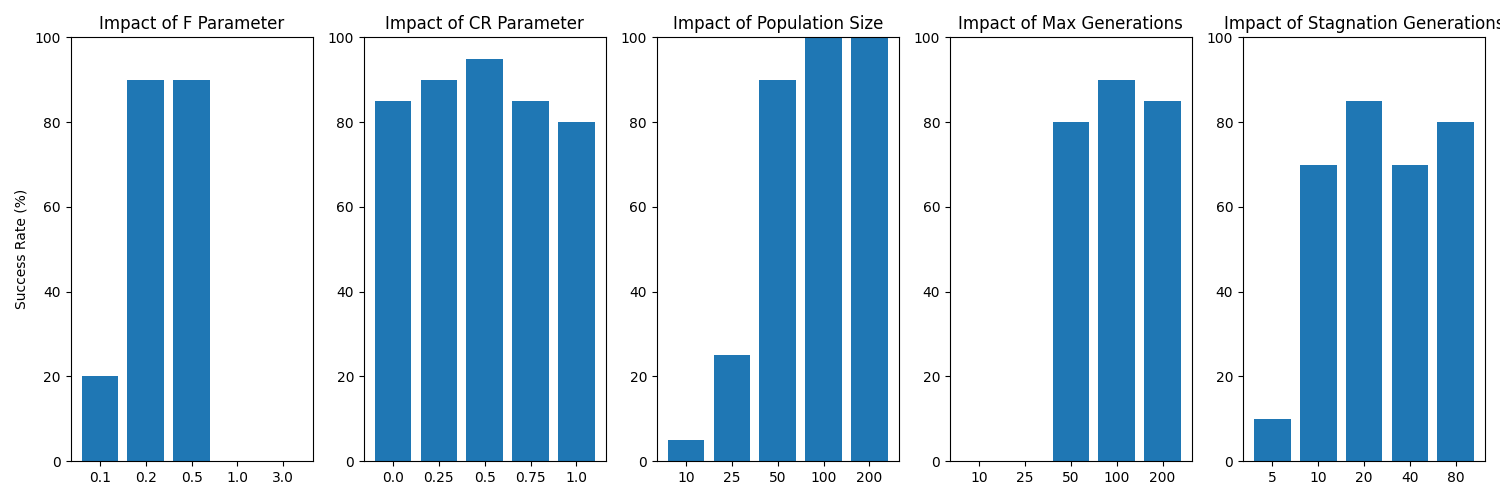
\includegraphics[width=\textwidth]{parameter_tuning_results_separate1.png}
    \caption{Wpływ parametrów na jakość algorytmu dla następujących wartości domyślnych: F = 0.5, CR = 0.5, wielkość populacji = 50, maksymalna liczba generacji = 100, stagnacja = 10}
    \label{fig:parameter_results1}
\end{figure}

\begin{figure}[H]
    \centering
    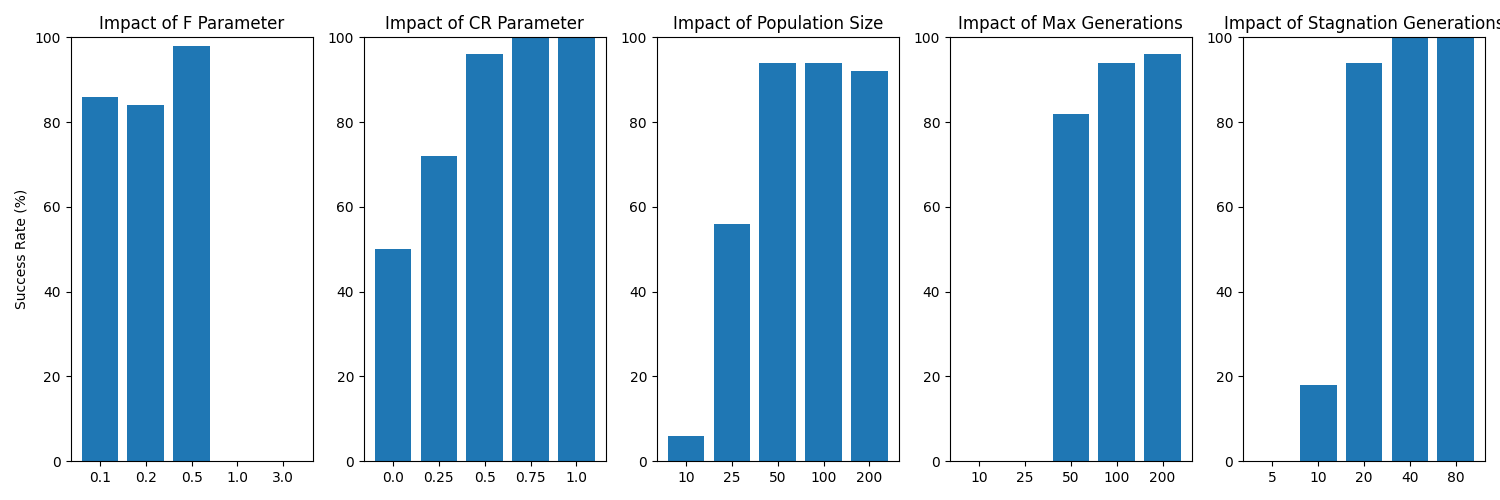
\includegraphics[width=\textwidth]{parameter_tuning_results_separate2.png}
    \caption{Wpływ parametrów na jakość algorytmu dla następujących wartości domyślnych: F = 0.5, CR = 0.5, wielkość populacji = 100, maksymalna liczba generacji = 100, stagnacja = 10}
    \label{fig:parameter_results2}
\end{figure}

\begin{figure}[H]
    \centering
    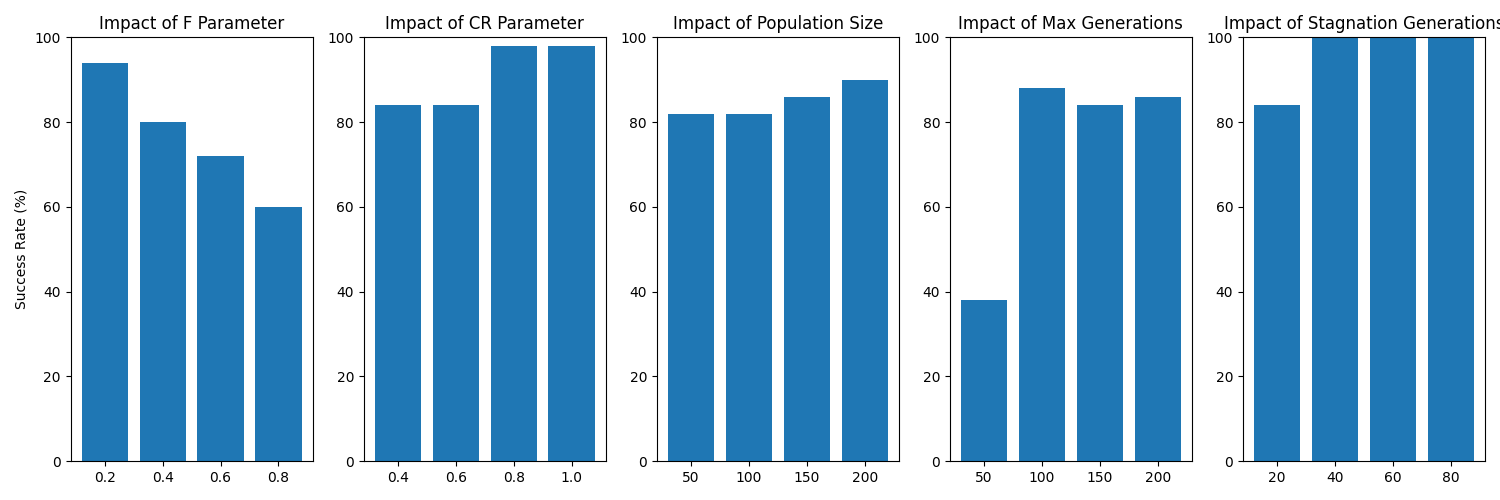
\includegraphics[width=\textwidth]{parameter_tuning_results_separate3.png}
    \caption{Wpływ parametrów na jakość algorytmu dla następujących wartości domyślnych: F = 0.5, CR = 0.5, wielkość populacji = 200, maksymalna liczba generacji = 100, stagnacja = 20}
    \label{fig:parameter_results3}
\end{figure}

\begin{figure}[H]
    \centering
    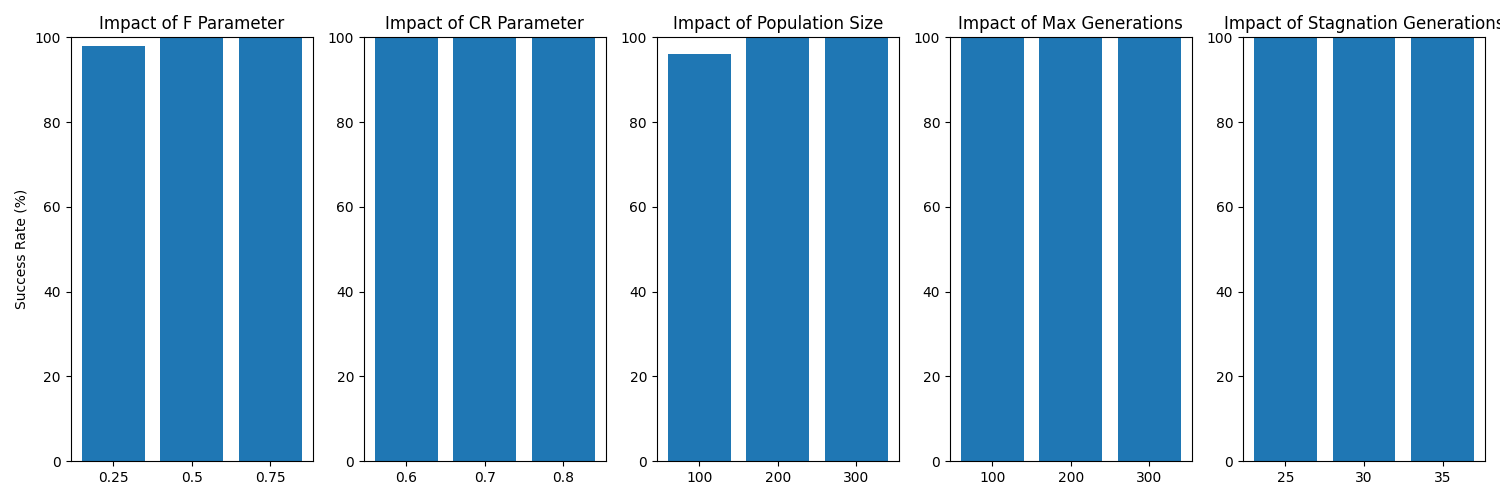
\includegraphics[width=\textwidth]{parameter_tuning_results_separate4.png}
    \caption{Wpływ parametrów na jakość algorytmu dla następujących wartości domyślnych: F = 0.5, CR = 0.8, wielkość populacji = 200, maksymalna liczba generacji = 100, stagnacja = 40}
    \label{fig:parameter_results4}
\end{figure}

Na podstawie przeprowadzonych eksperymentów wyznaczyliśmy optymalne wartości parametrów algorytmu ewolucji różnicowej:
\begin{enumerate}
    \item F - 0.5
    \item CR - 0.7
    \item Wielkość populacji - 200
    \item Maksymalna liczba generacji - 300
    \item Stagnacja - 30
\end{enumerate}


\section{Model zastępczy}
W ramach projektu jako model zastępczy stworzyliśmy drzewo regresyjne. Model wykorzystuje algorytm minimalizacji błędu średniokwadratowego (MSE), pozwalając na kontrolę głębokości drzewa i minimalnej liczby próbek w liściach. Implementacja znajduje się w pliku custom\_tree.py.

Proces trenowania modelu DecisionTreeRegressor jest realizowany poprzez rekurencyjne budowanie struktury drzewa, gdzie każdy węzeł reprezentuje punkt decyzyjny oparty na wartości konkretnej cechy.  Proces zaczyna się od inicjalizacji drzewa z określonymi parametrami kontrolującymi jego wzrost. Głównym elementem procesu trenowania jest procedura budowy drzewa, która rozpoczyna się od korzenia i rekurencyjnie tworzy kolejne węzły. W każdym węźle algorytm musi podjąć decyzję: czy utworzyć liść, czy kontynuować podział. Decyzja ta jest podejmowana na podstawie warunków stopu: osiągnięcie maksymalnej głębokości lub zbyt mała liczba próbek.

Jeśli podział jest możliwy, algorytm poszukuje najlepszego sposobu podziału danych poprzez iterowanie po wszystkich dostępnych cechach i potencjalnych progach podziału. Dla każdej kombinacji cechy i progu obliczany jest błąd średniokwadratowy powstałych podzbiorów. Wybierany jest podział minimalizujący sumę błędów obu powstałych grup.

Aby zwiększyć wydajność, progi podziału nie są wybierane ze wszystkich możliwych wartości cechy, lecz z wybranych percentyli, co znacząco redukuje przestrzeń poszukiwań. Implementacja wykorzystuje również operacje zwektoryzowane numpy, co przyspiesza obliczenia w porównaniu do tradycyjnych pętli.

Po znalezieniu najlepszego podziału, dane dzielone są na dwie grupy, a proces jest rekurencyjnie powtarzany dla każdej z nich. Tworzy to strukturę drzewiastą, gdzie każdy węzeł wewnętrzny zawiera regułę podziału (cechę i próg), a każdy liść wartość przewidywaną - średnią wartość zmiennej celu dla próbek, które trafiły do tego liścia.

Dzięki takiej strukturze można przewidywać wartości dla nowych próbek. Proces predykcji polega na przejściu od korzenia do odpowiedniego liścia, kierując się w każdym węźle regułami podziału i zwróceniu wartości zapisanej w liściu.

Model inicjowany jest 3 parametrami:
\begin{enumerate}
    \item Maksymalna głębokość drzewa.
    \item Minimalna liczba próbek do podziału.
    \item Minimalna liczba próbek w liściu.
\end{enumerate}

Podczas inicjacji do historii dodawane są punkty z początkowej populacji.
Model trenowany jest całą historią próbek przy każdej generacji populacji (wymagane jest zadane minimum próbek treningowych). Do historii dodawane są punkty z każdej faktycznej ewaluacji funkcji celu.
Model wykorzystywany jest do predykcji wartości dla wszystkich nowych kandydatów. Parametr ewolucji różnicowej top\_percentage odpowiada za określenie ile procent najlepszych przewidywanych rozwiązań będzie rzeczywiście ewaluowanych. Historia zewaluowanych punktów nie ma ograniczonego rozmiaru, a dodane do niej punkty nie są usuwane. Zapewnia to pełną informację o przestrzeniu przeszukiwań.

\subsection{Wyznaczanie parametrów drzewa regresyjnego}

Aby wyznaczyć optymalne parametry drzewa regresyjnego, algorytm uruchomiliśmy dla dwuwymiarowej wersji funkcji Shifted Rotated Griewank z benchmarku CEC. Wyznaczyliśmy parametry drzewa regresyjnego w ten sam sposób, co parametry ewolucji różnicowej - poprzez testowanie pojedynczych parametrów dla domyślnych wartości pozostałych parametrów.

\begin{figure}[H]
    \centering
    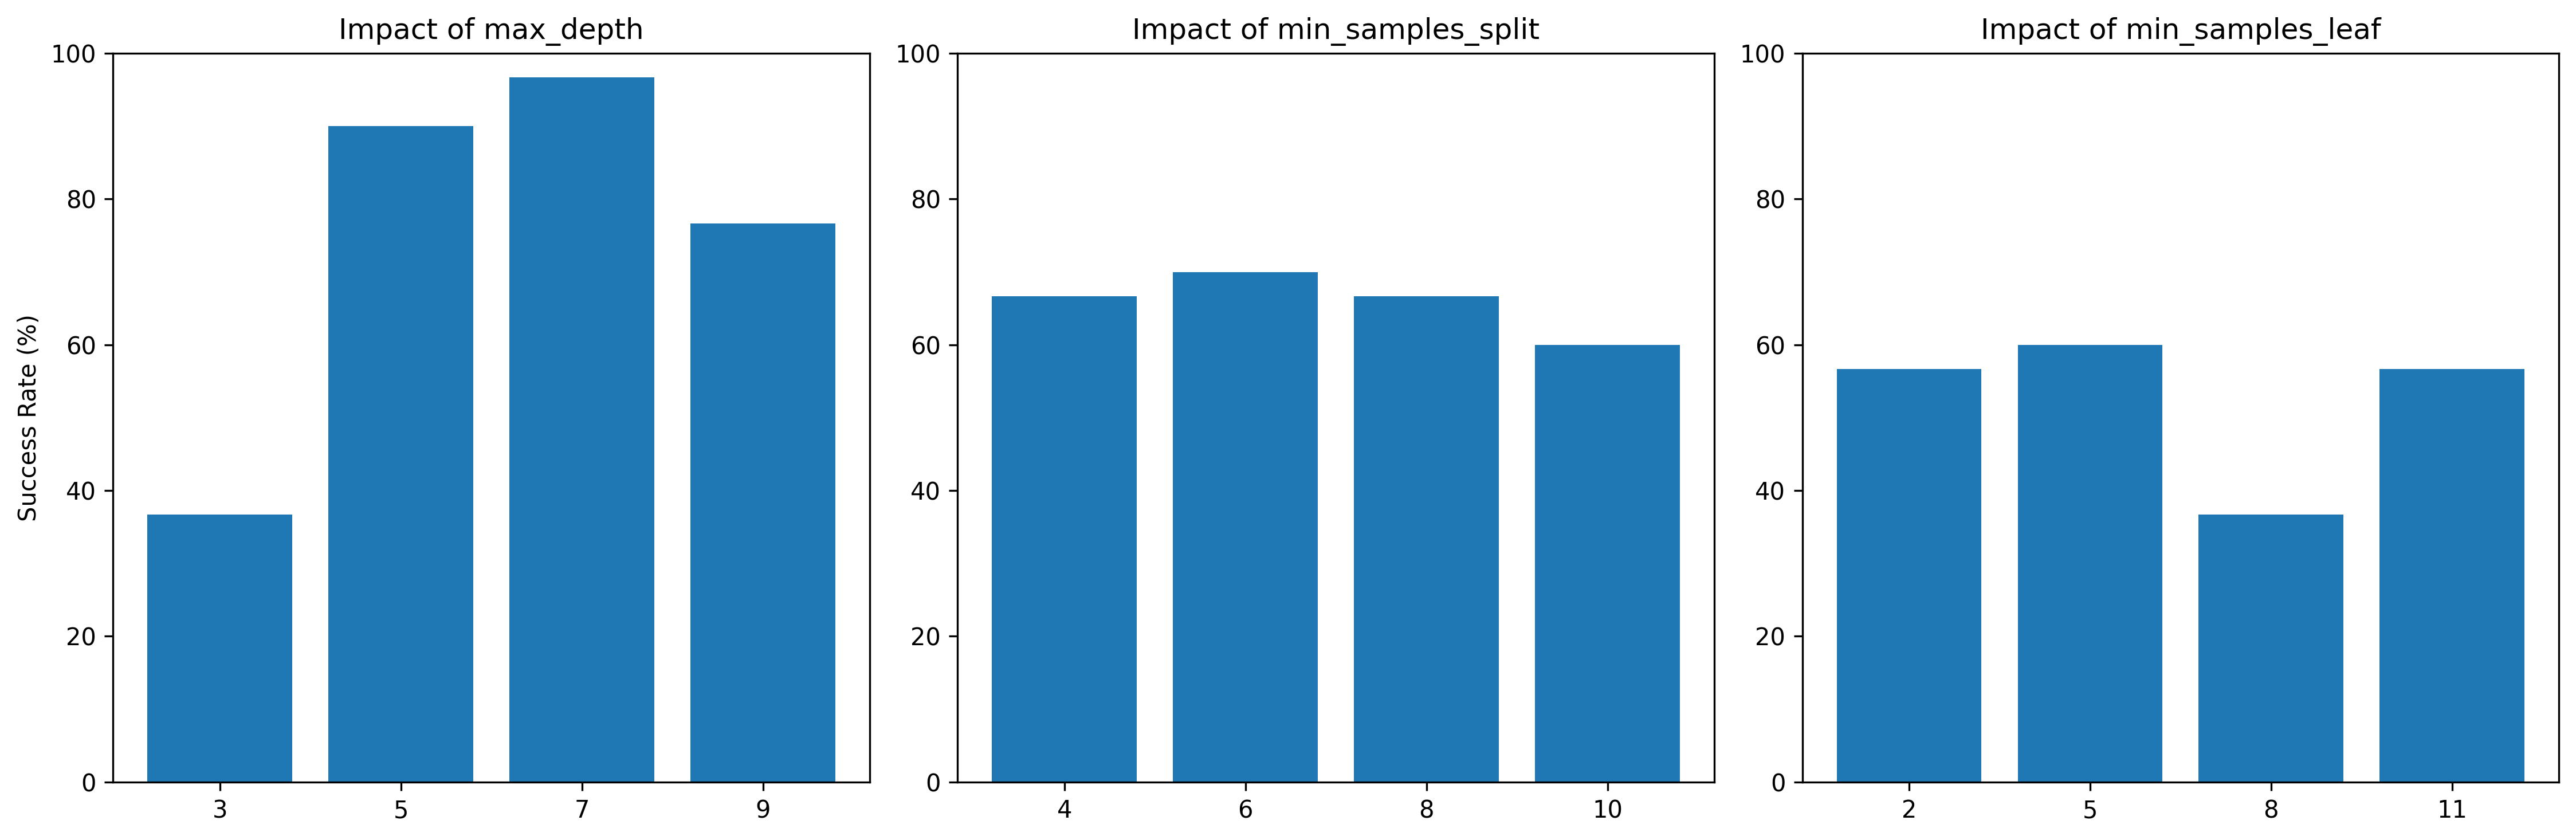
\includegraphics[width=\textwidth]{tree_parameter_tuning_separate_results2.png}
    \caption{Wpływ parametrów drzewa regresyjnego na skuteczność działania algorytmu dla następujących wartości domyślnych: maksymalna głębokość = 10, minimalna liczba próbek do podziału = 1, minimalna liczba próbek w liściu = 3}
    \label{fig:tree_parameter_results1}
\end{figure}

\begin{figure}[H]
    \centering
    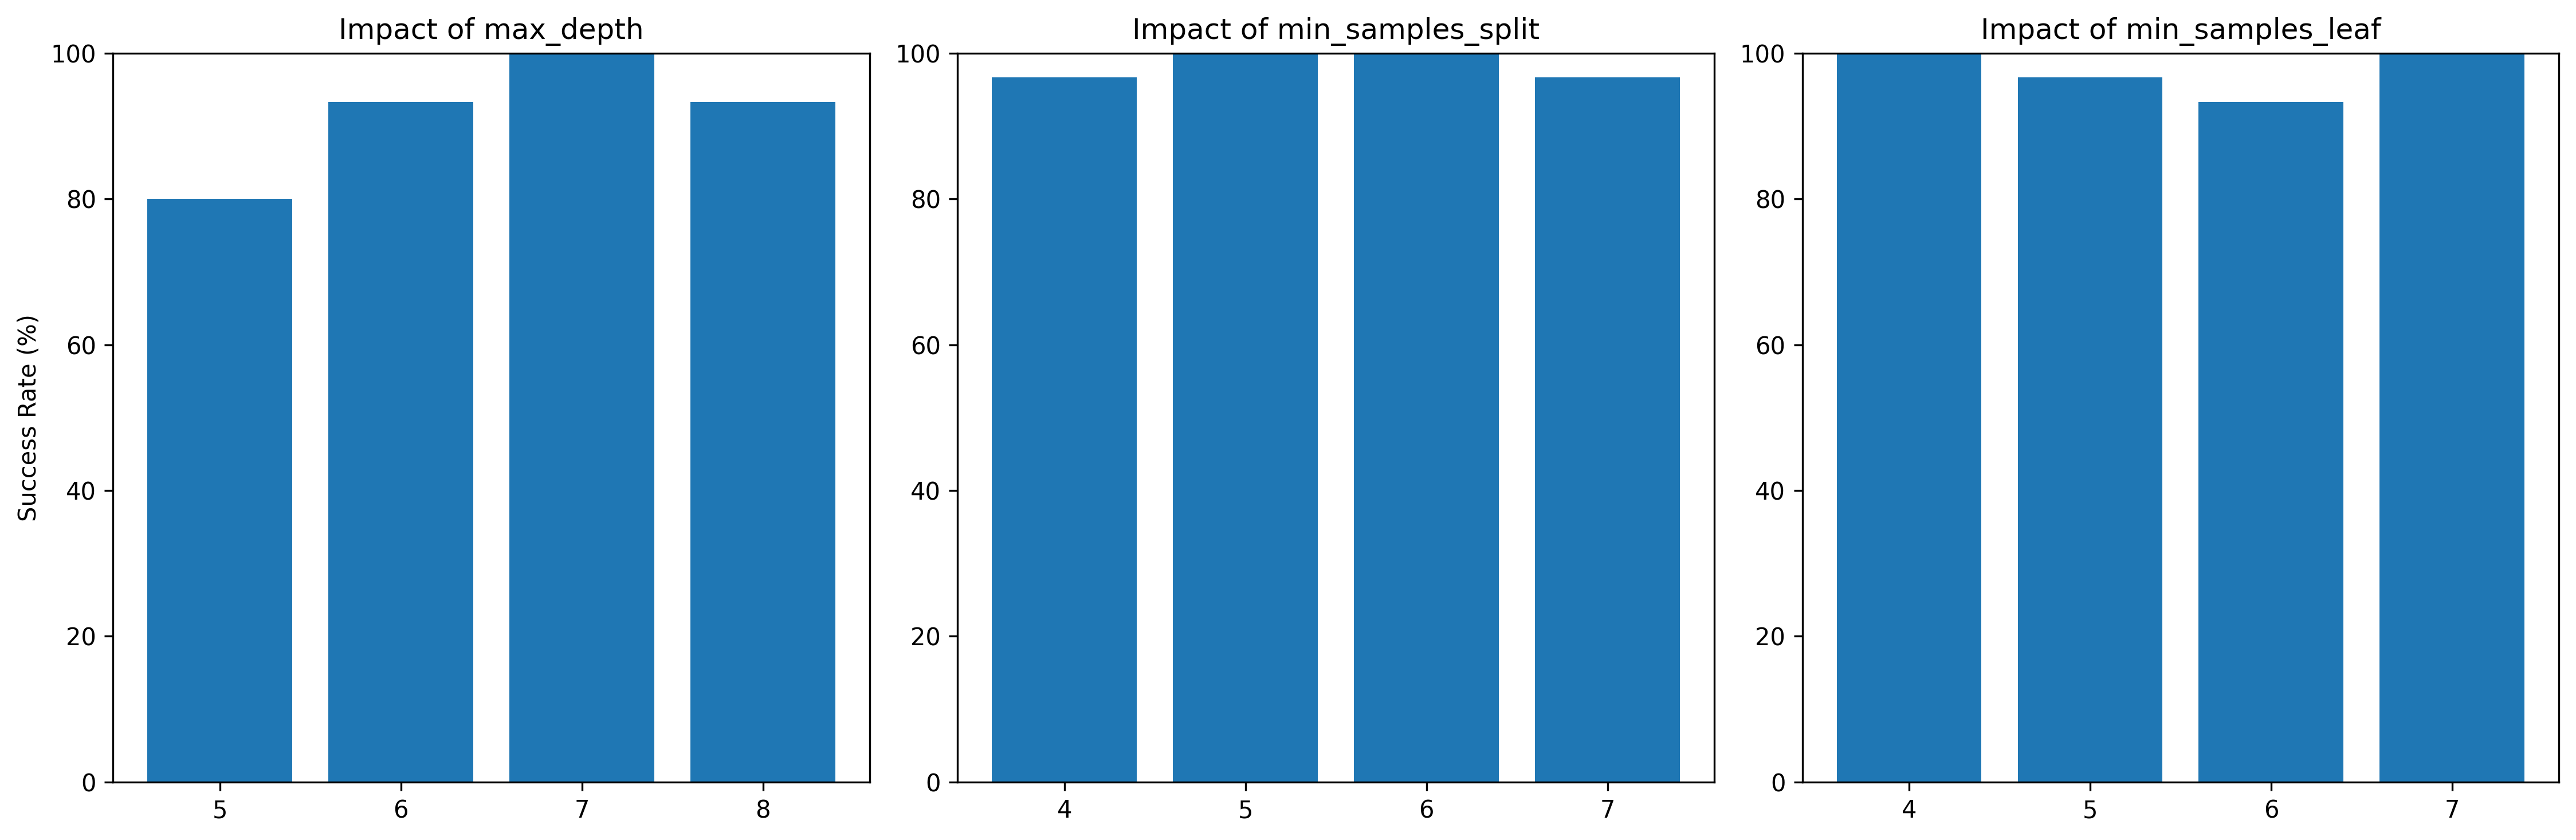
\includegraphics[width=\textwidth]{tree_parameter_tuning_separate_results3.png}
    \caption{Wpływ parametrów drzewa regresyjnego na skuteczność działania algorytmu dla następujących wartości domyślnych: maksymalna głębokość = 7, minimalna liczba próbek do podziału = 5, minimalna liczba próbek w liściu = 4}
    \label{fig:tree_parameter_results2}
\end{figure}

Na podstawie przeprowadzonych eksperymentów udało nam się wyznaczyć optymalne parametry drzewa regresyjnego:

\begin{enumerate}
    \item Maksymalna głębokość - 7
    \item Minimalna liczba próbek do podziału - 5
    \item Minimalna liczba próbek w liściu - 4
\end{enumerate}

Ostatnie dwa parametry, które przetestowaliśmy w celu uzyskania jak najleszych wyników to:
\begin{enumerate}
    \item procent najlepszych rozwiązań, które będą ewaluowane
    \item częstotliwość uczenia modelu zastępczego - co ile generacji model będzie trenowany na nowych danych
\end{enumerate}

Na podstawie ekperymentów, których wyniki zostały przedstawione poniżej, udało nam się wyznaczyć optymalne wartości tych parametrów:
\begin{enumerate}
    \item procent najlepszych rozwiązań, które będą ewaluowane - 0.65
    \item częstotliwość uczenia modelu zastępczego - 16
\end{enumerate}

Dla wartości większych niż powyższe algorytm zwacał porównywalne wyniki, jednak kosztem większej ilości ewaluacji funkcji celu. Dla wartości mniejszych niż powyższe algortm zwracał gorsze wyniki.

\begin{figure}[H]
    \centering
    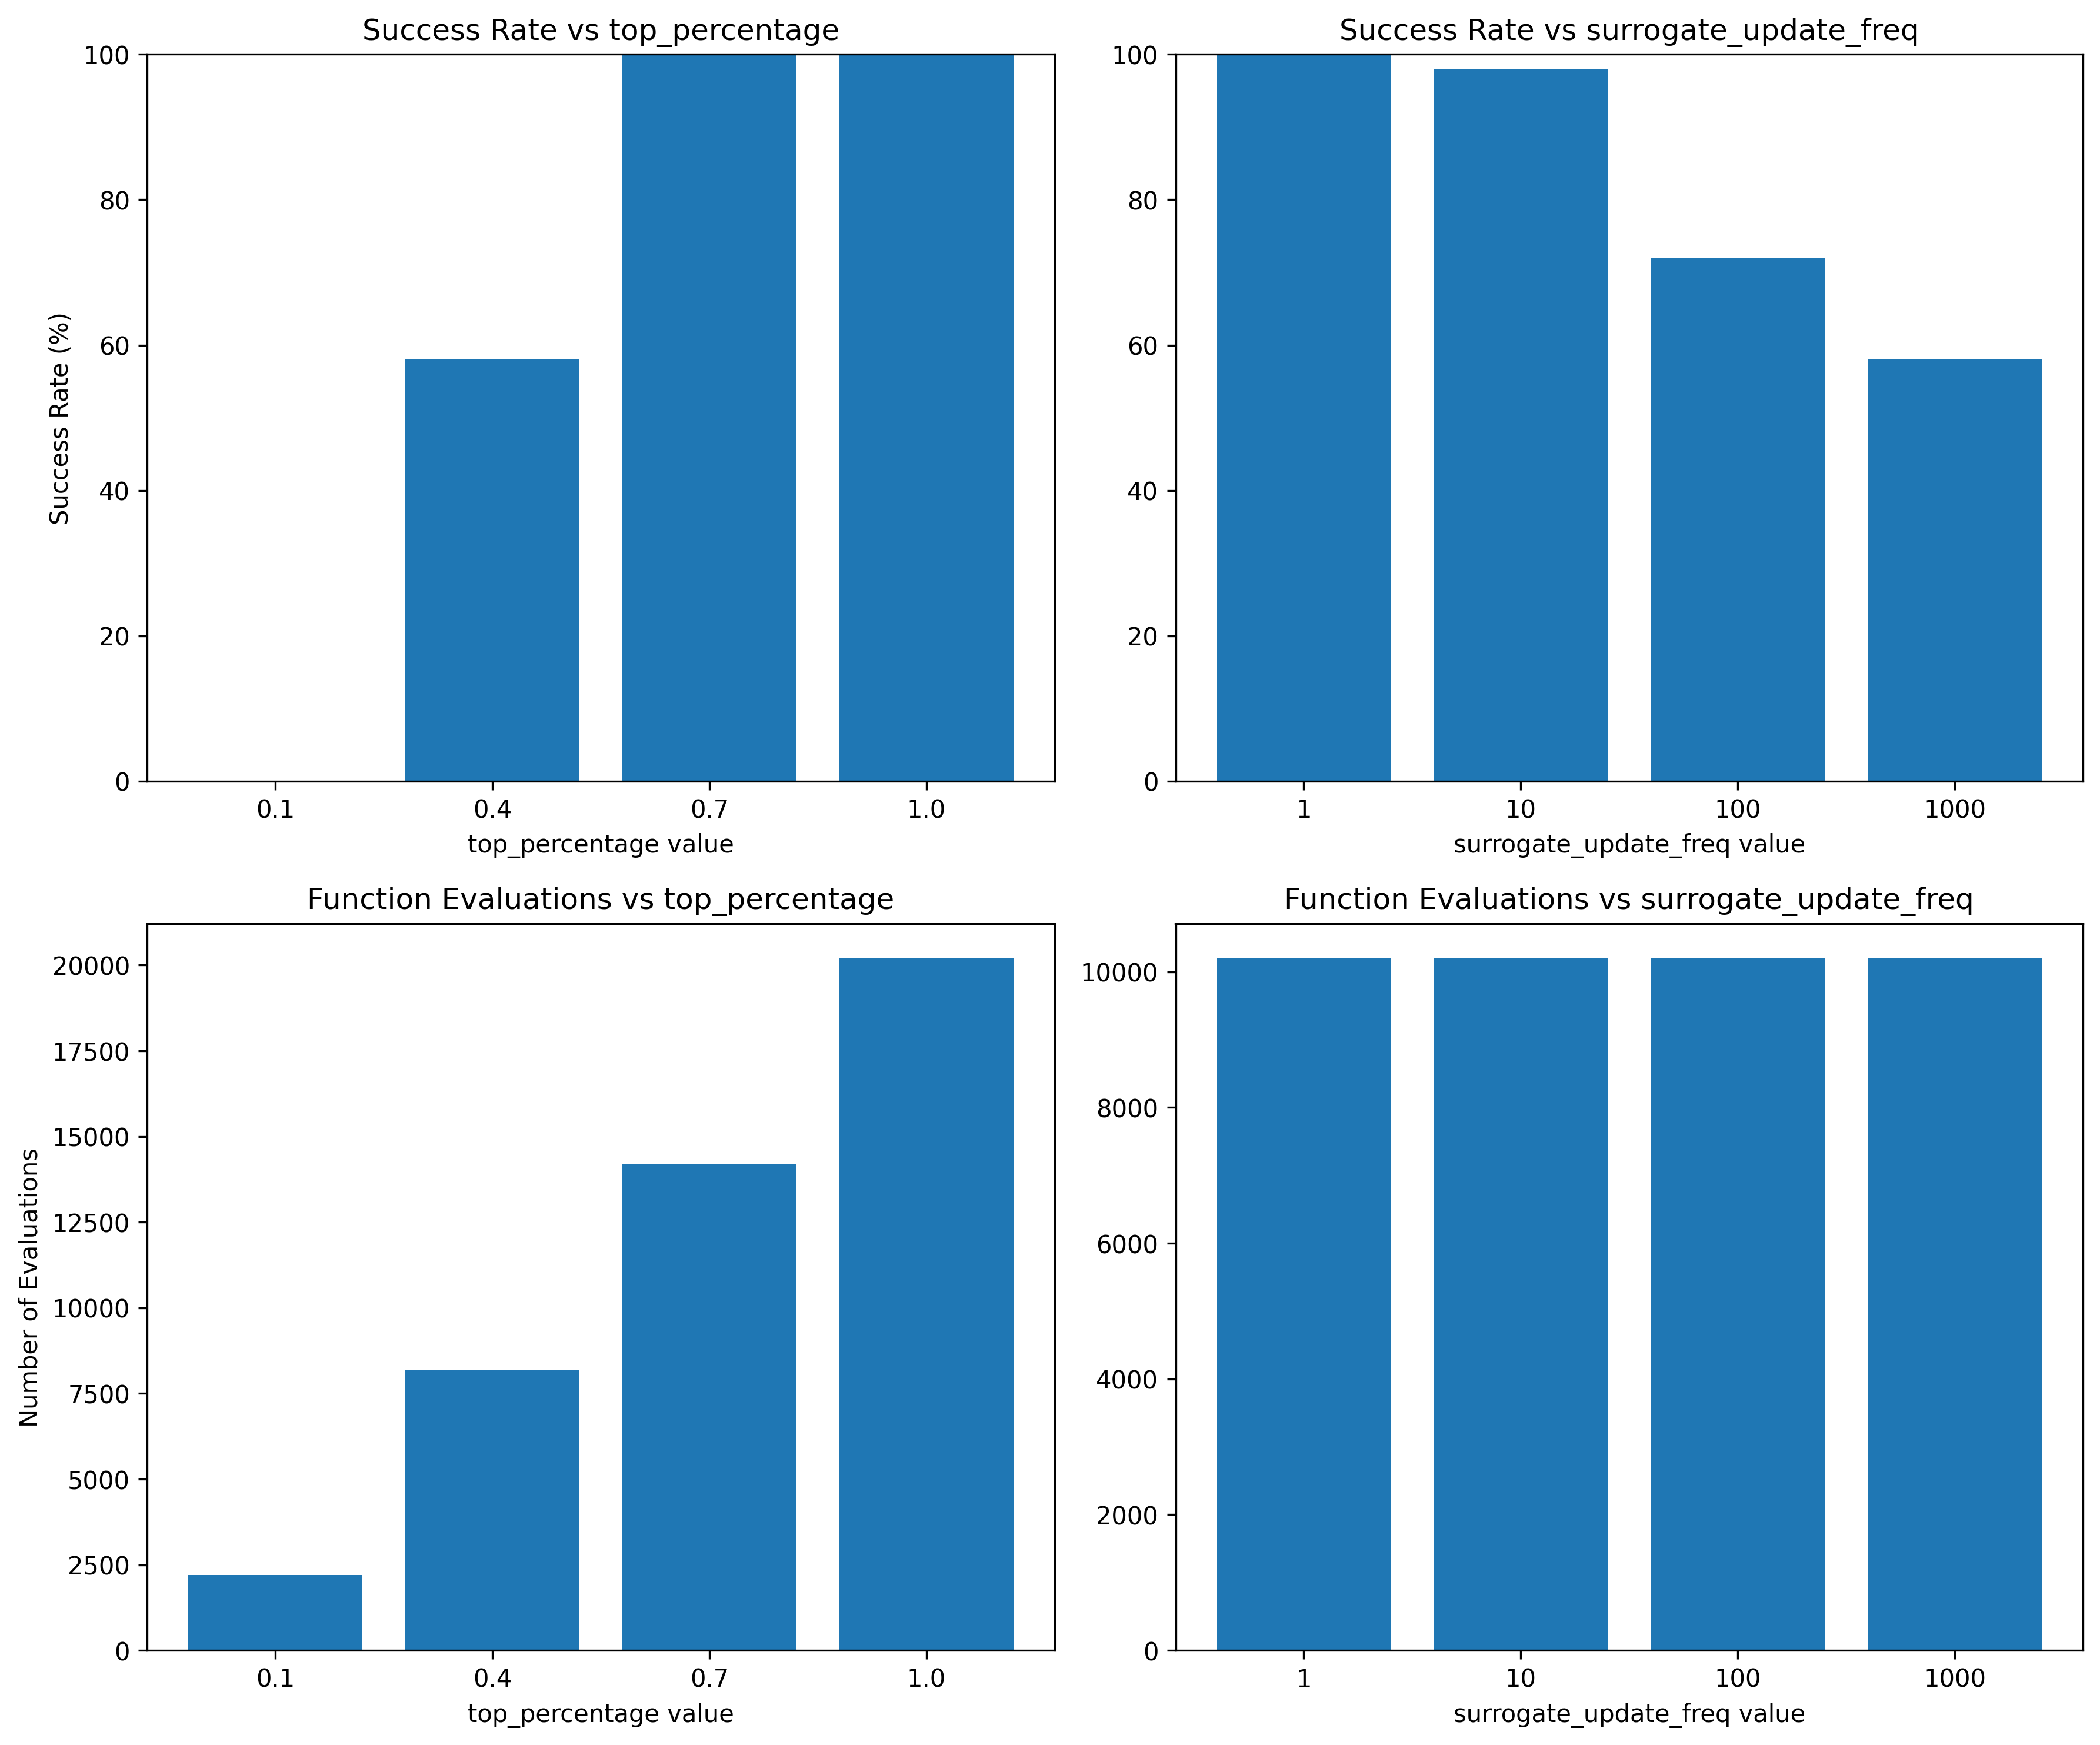
\includegraphics[width=\textwidth]{surrogate_de_parameter_tuning_results1.png}
    \caption{Wpływ procentu najlepszych rozwiązań, które są ewaluowane oraz częstotliwości uczenia modelu na skuteczność działania algorytmu dla następujących wartości domyślnych: procent najlepszych rozwiązań = 0.5, częstotliwość uczenia = 5}
    \label{fig:surogate_de_parameter_results1}
\end{figure}

\begin{figure}[H]
    \centering
    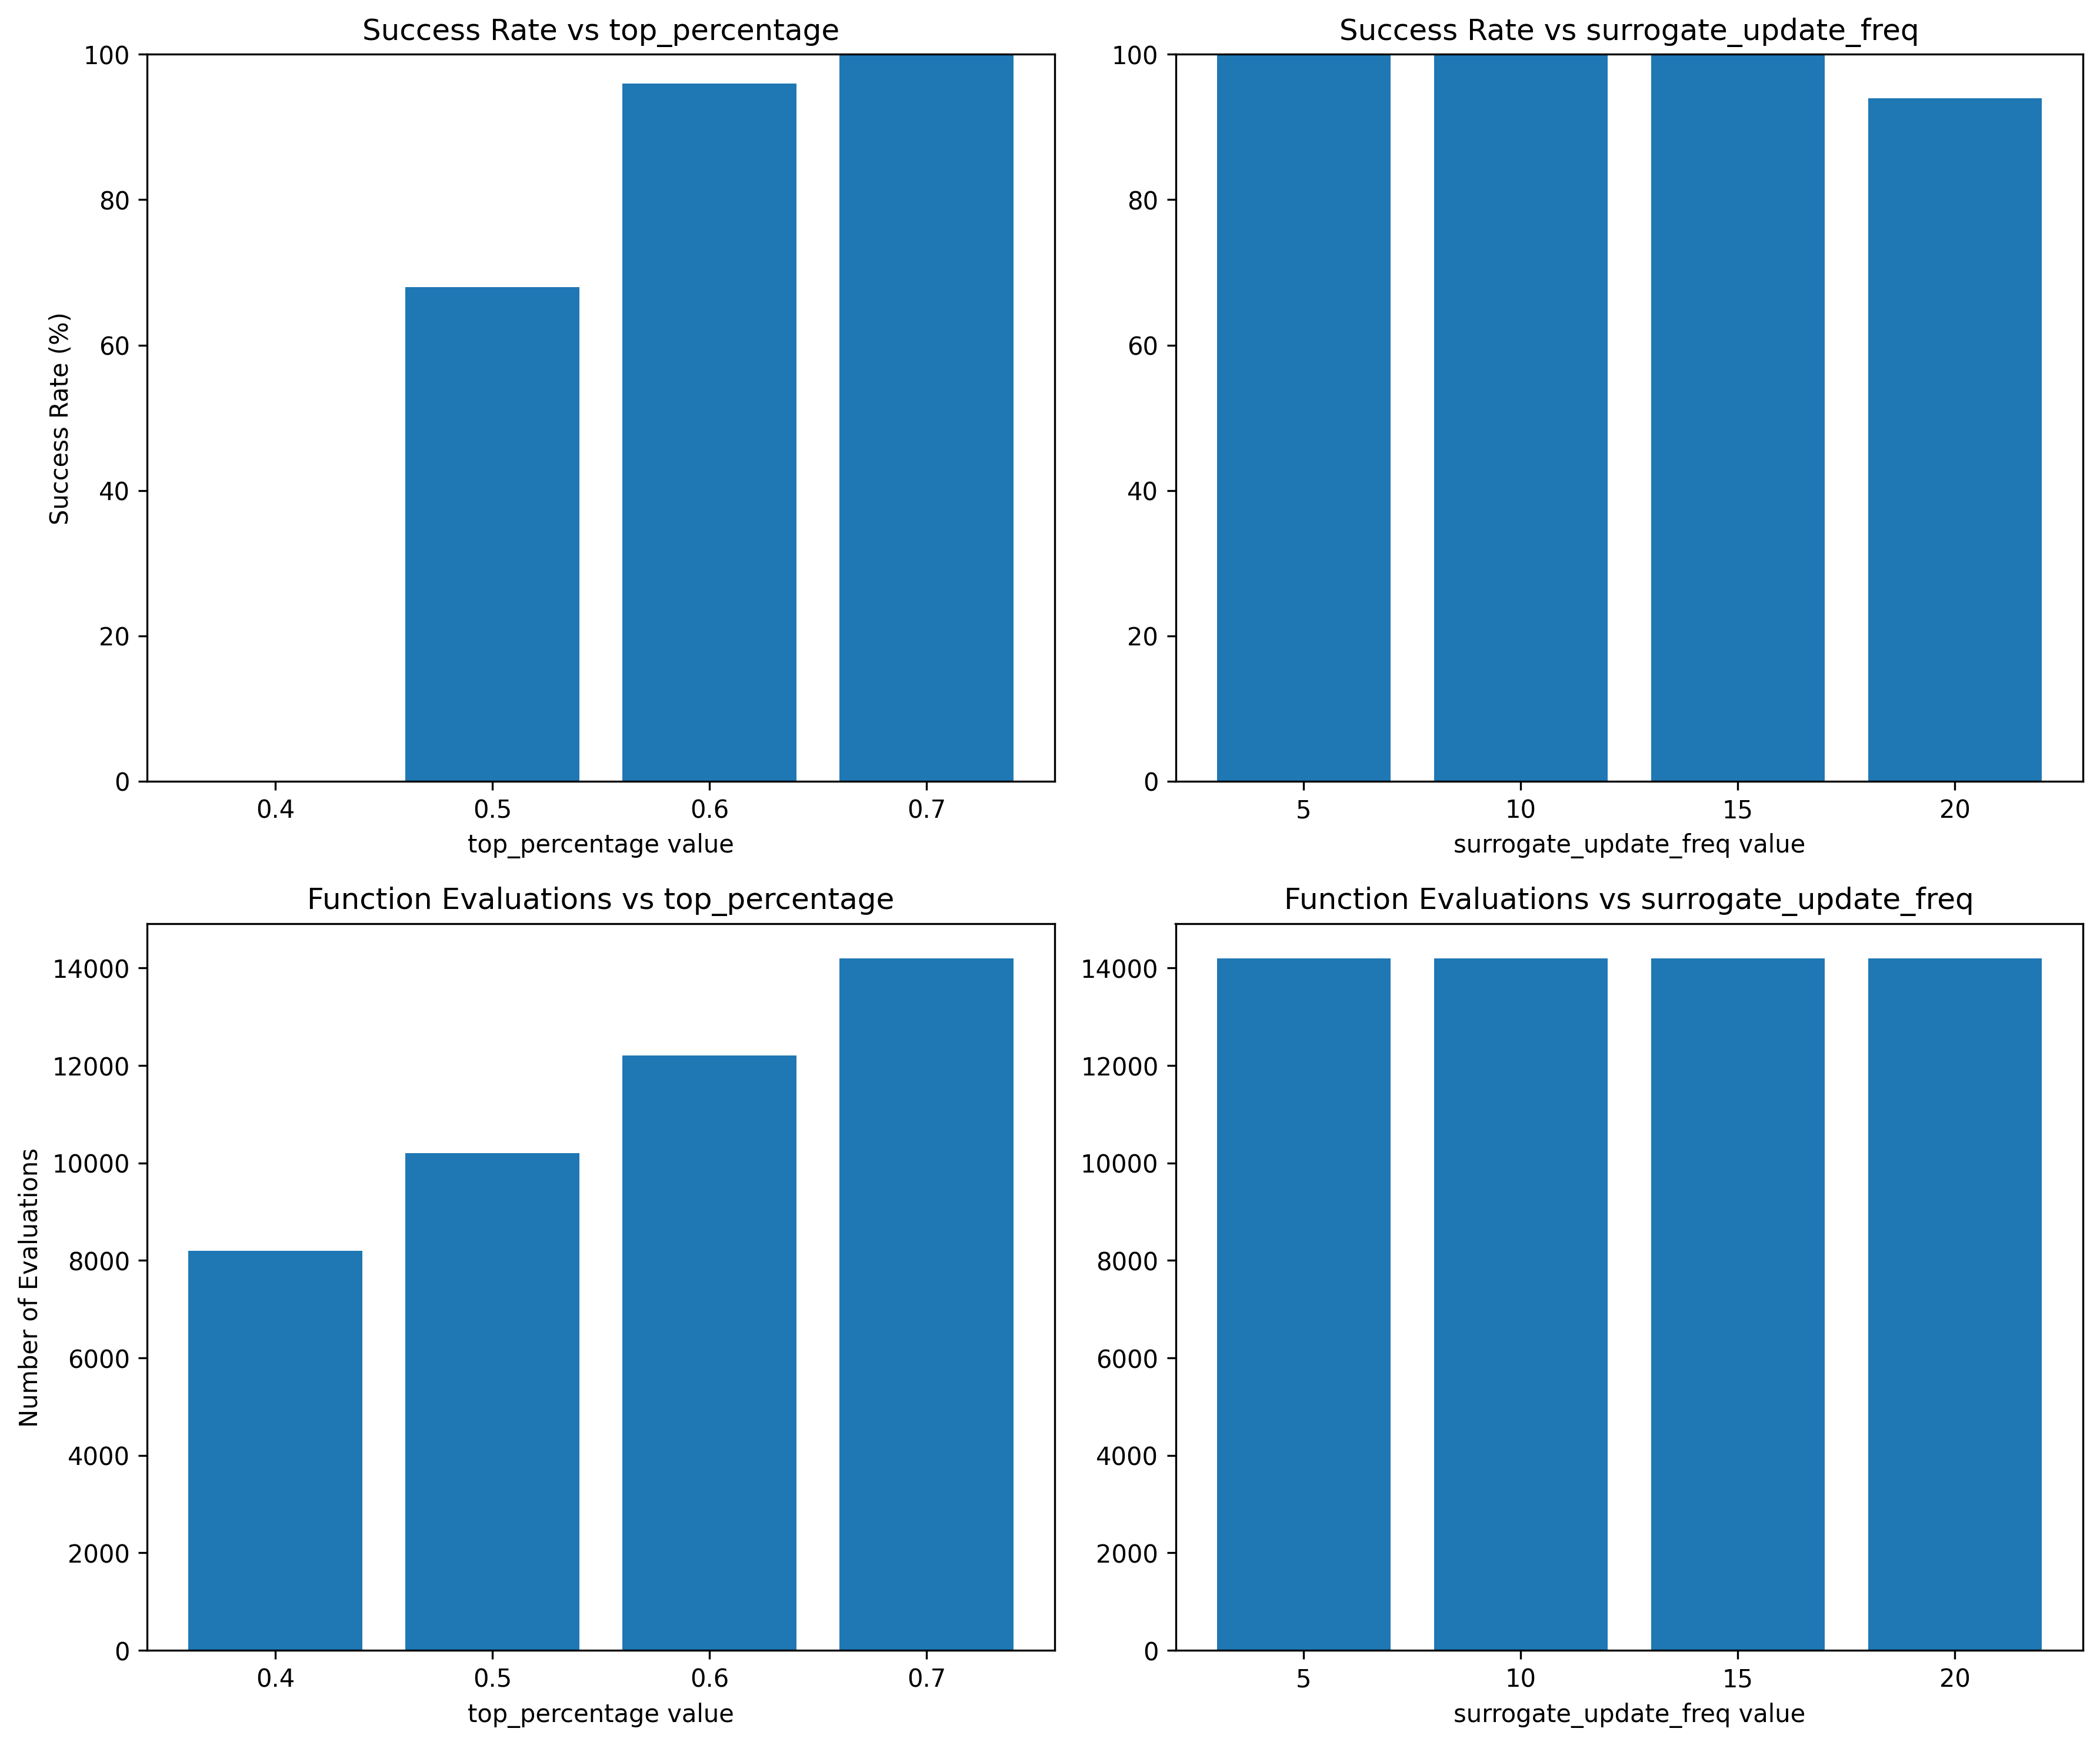
\includegraphics[width=\textwidth]{surrogate_de_parameter_tuning_results2.png}
    \caption{Wpływ procentu najlepszych rozwiązań, które są ewaluowane oraz częstotliwości uczenia modelu na skuteczność działania algorytmu dla następujących wartości domyślnych: procent najlepszych rozwiązań = 0.7, częstotliwość uczenia = 10}
    \label{fig:surogate_de_parameter_results2}
\end{figure}

\begin{figure}[H]
    \centering
    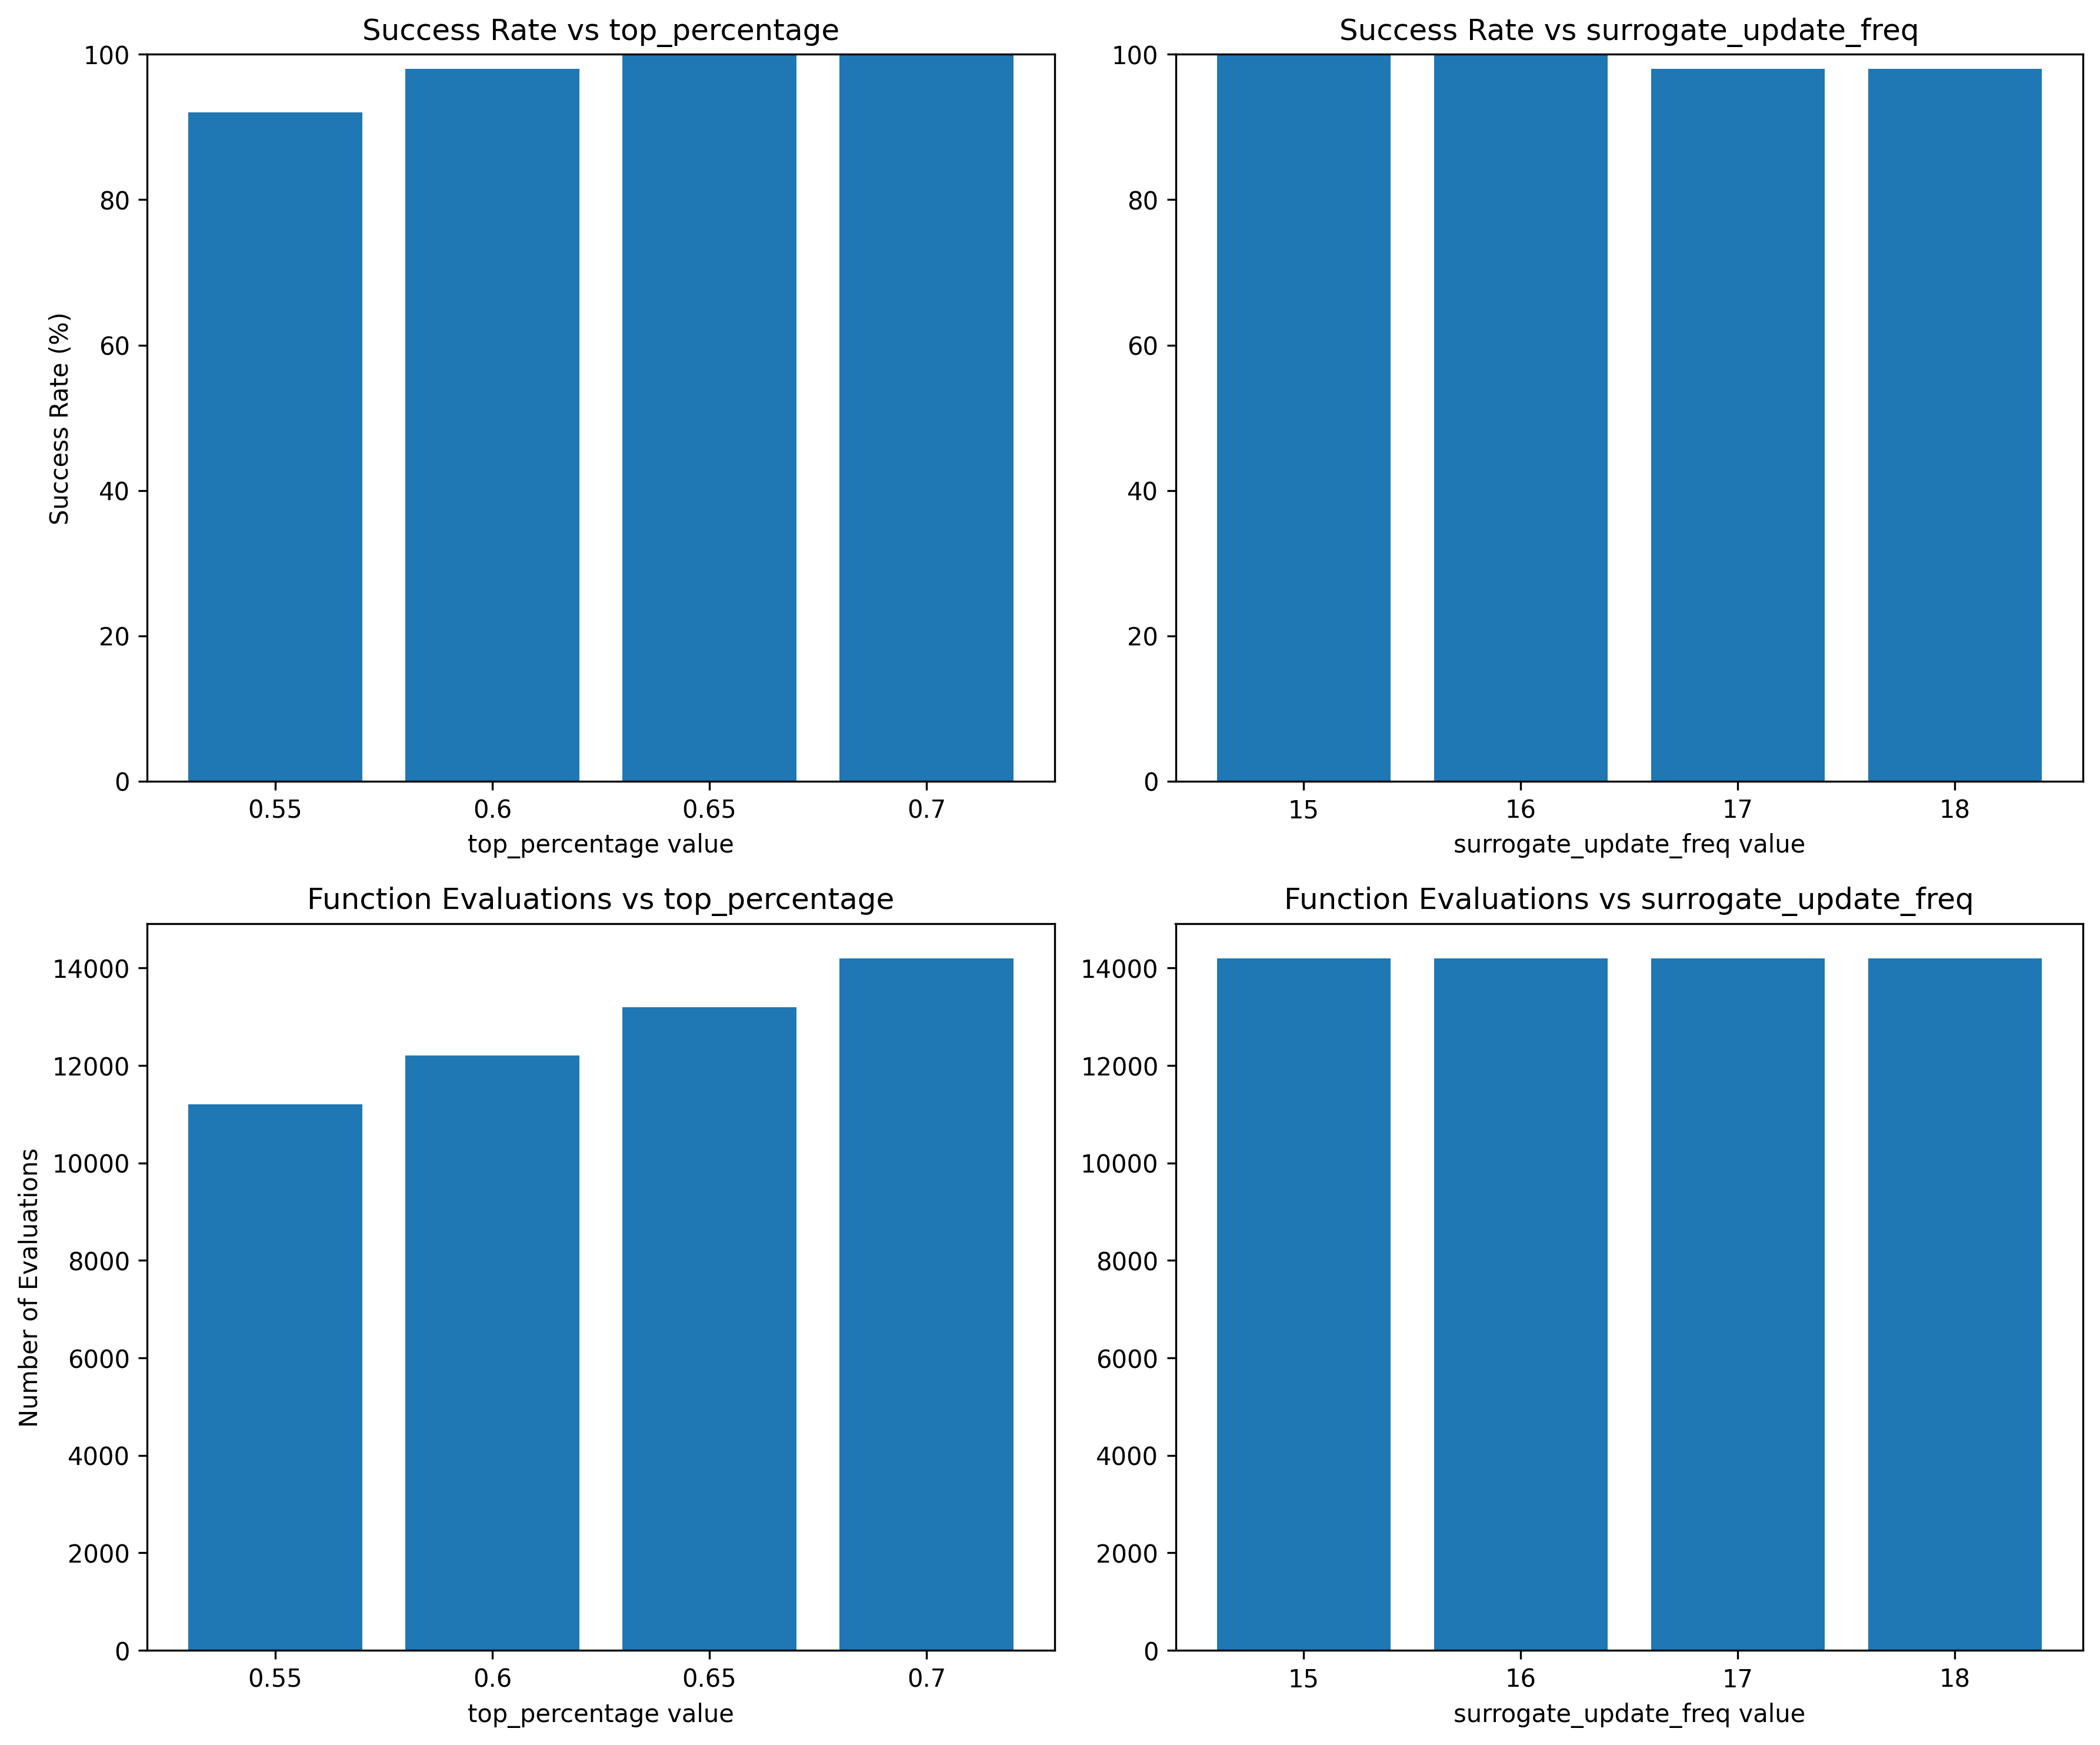
\includegraphics[width=\textwidth]{surrogate_de_parameter_tuning_results3.png}
    \caption{Wpływ procentu najlepszych rozwiązań, które są ewaluowane oraz częstotliwości uczenia modelu na skuteczność działania algorytmu dla następujących wartości domyślnych: procent najlepszych rozwiązań = 0.7, częstotliwość uczenia = 15}
    \label{fig:surogate_de_parameter_results3}
\end{figure}

\section{Porównanie wydajności}

Do testowania algorytmów wykorzystaliśmy dwuwymiarowe funkcje testowe z benchmarku CEC: Shifted Sphere, Shifted Schwefel, Shifted Rotated Elliptic oraz Shifted Rotated Griewank. Każda z nich miała optimum globalne wynoszące 0.

\begin{figure}[H]
    \centering
    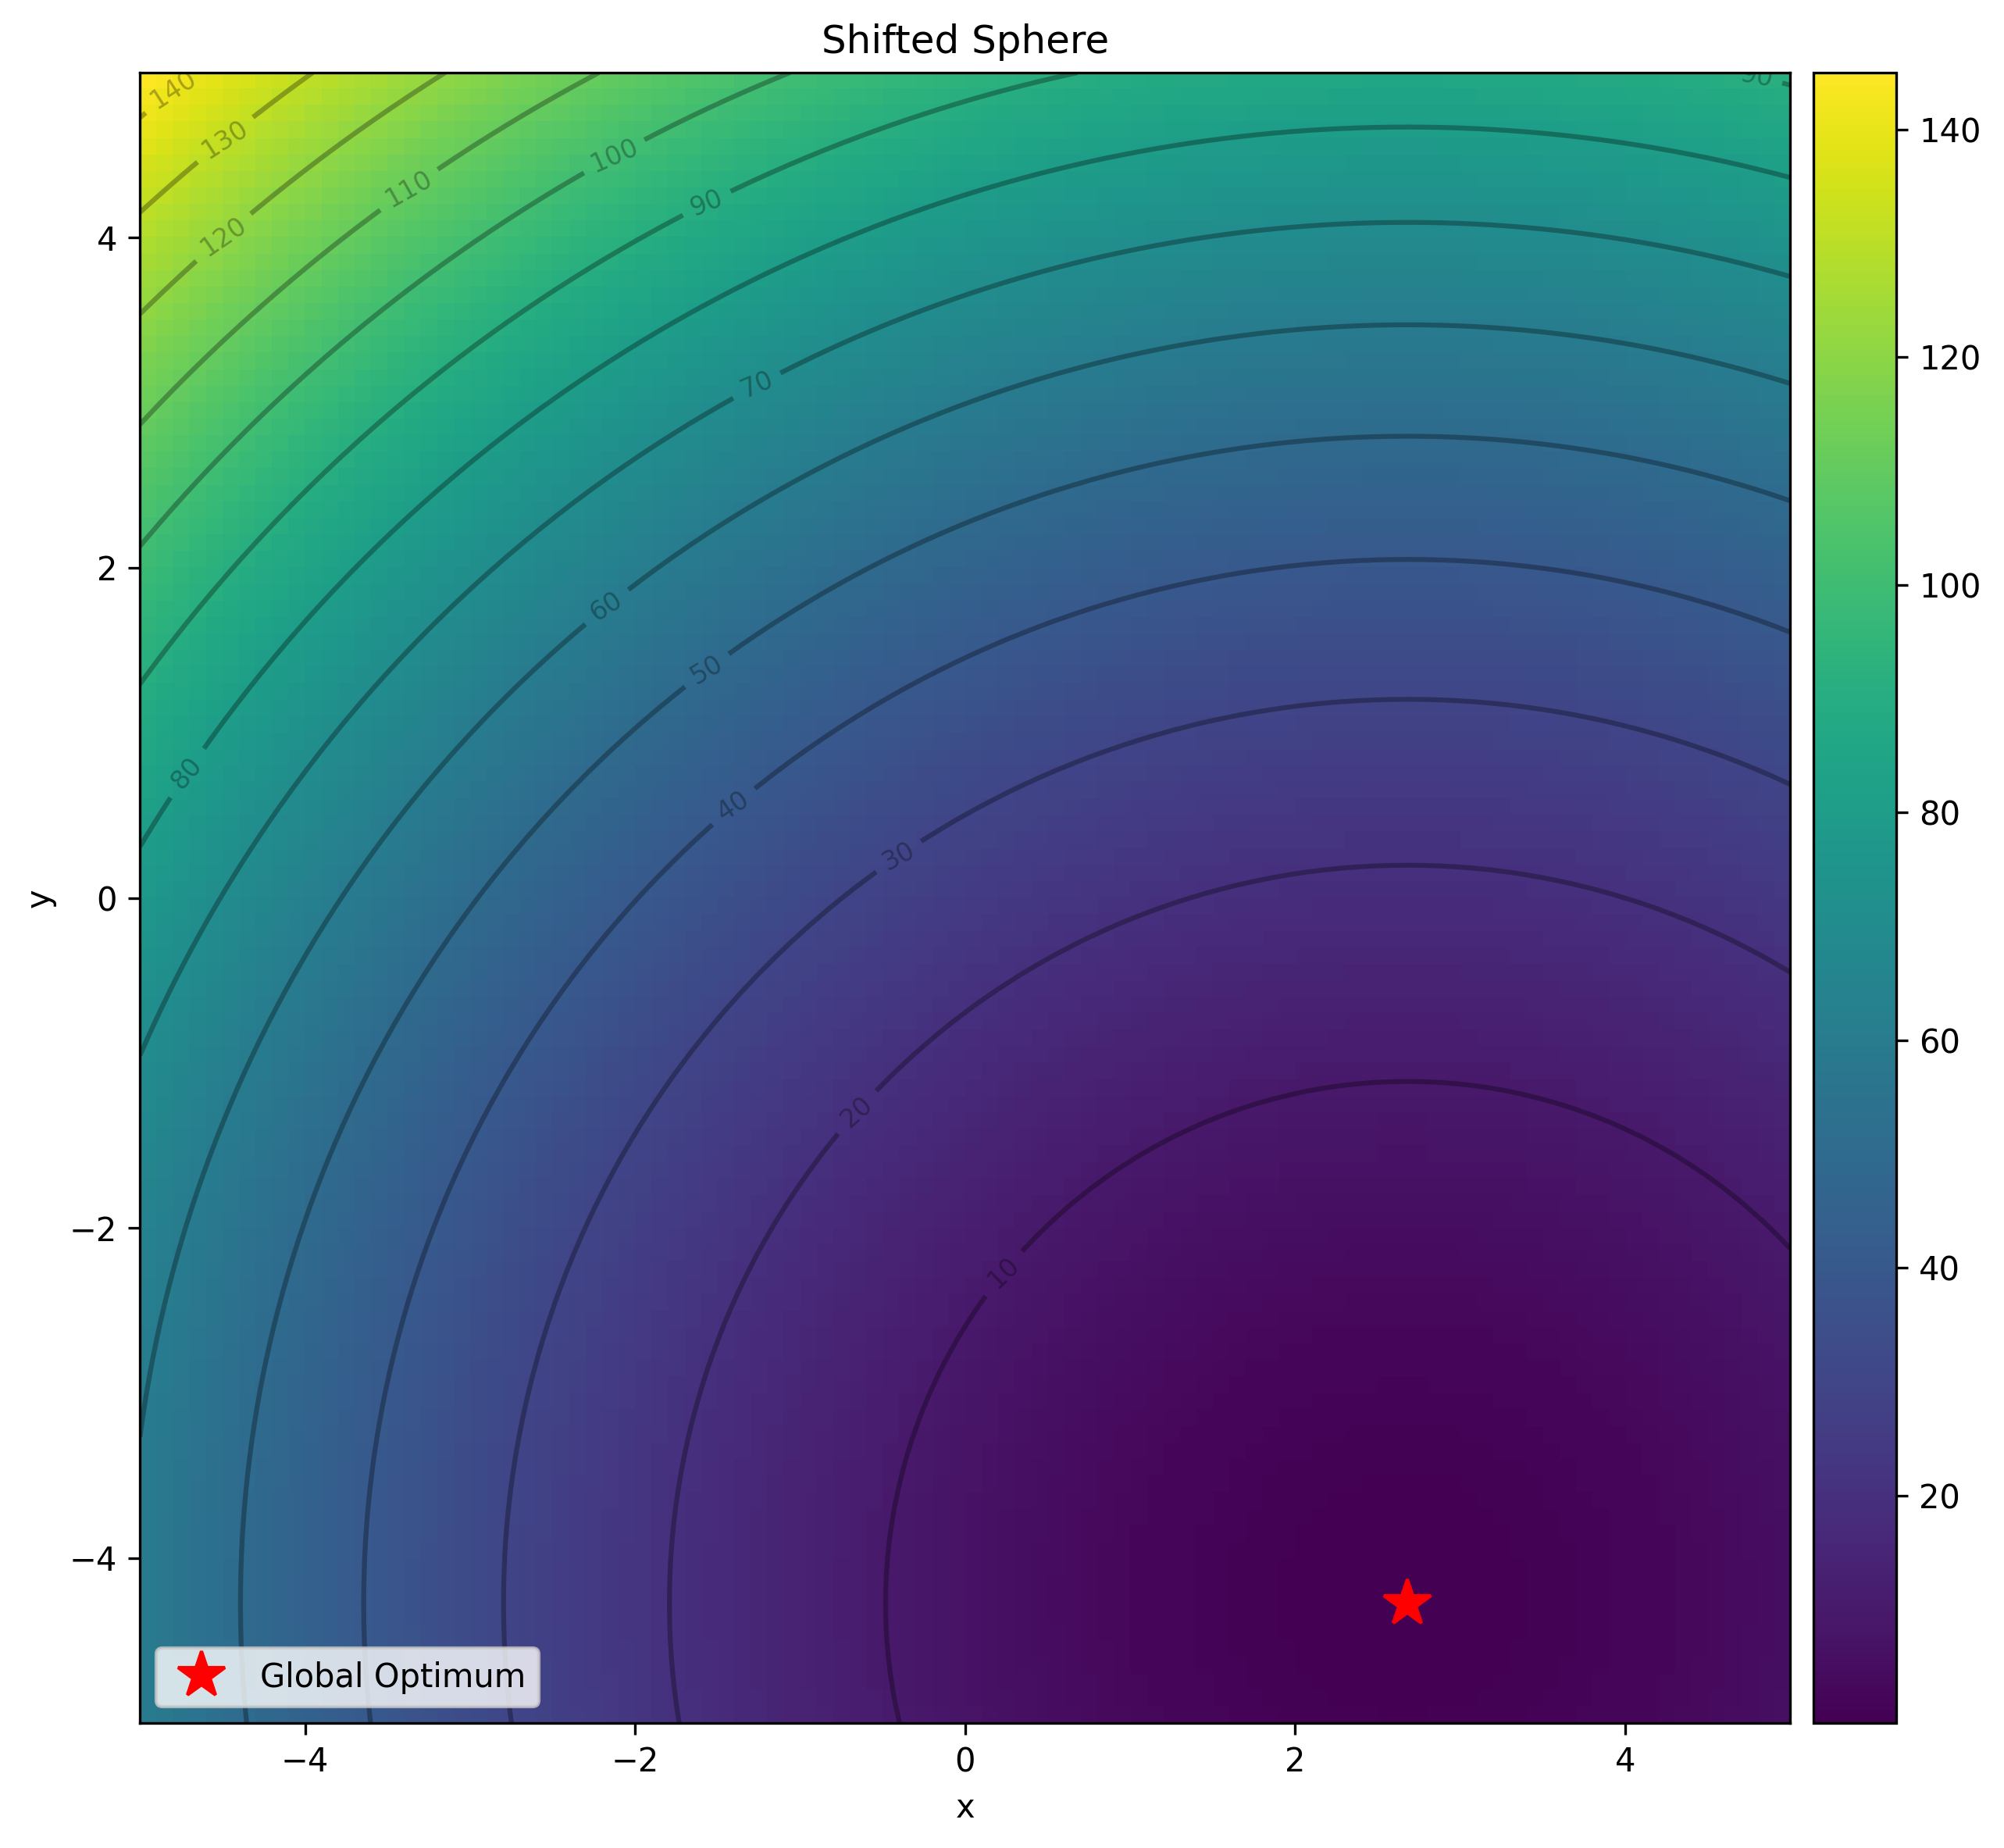
\includegraphics[width=\textwidth]{shifted_sphere.png}
    \caption{Wykres funkcji Shifted Sphere}
    \label{fig:plot1}
\end{figure}

\begin{figure}[H]
    \centering
    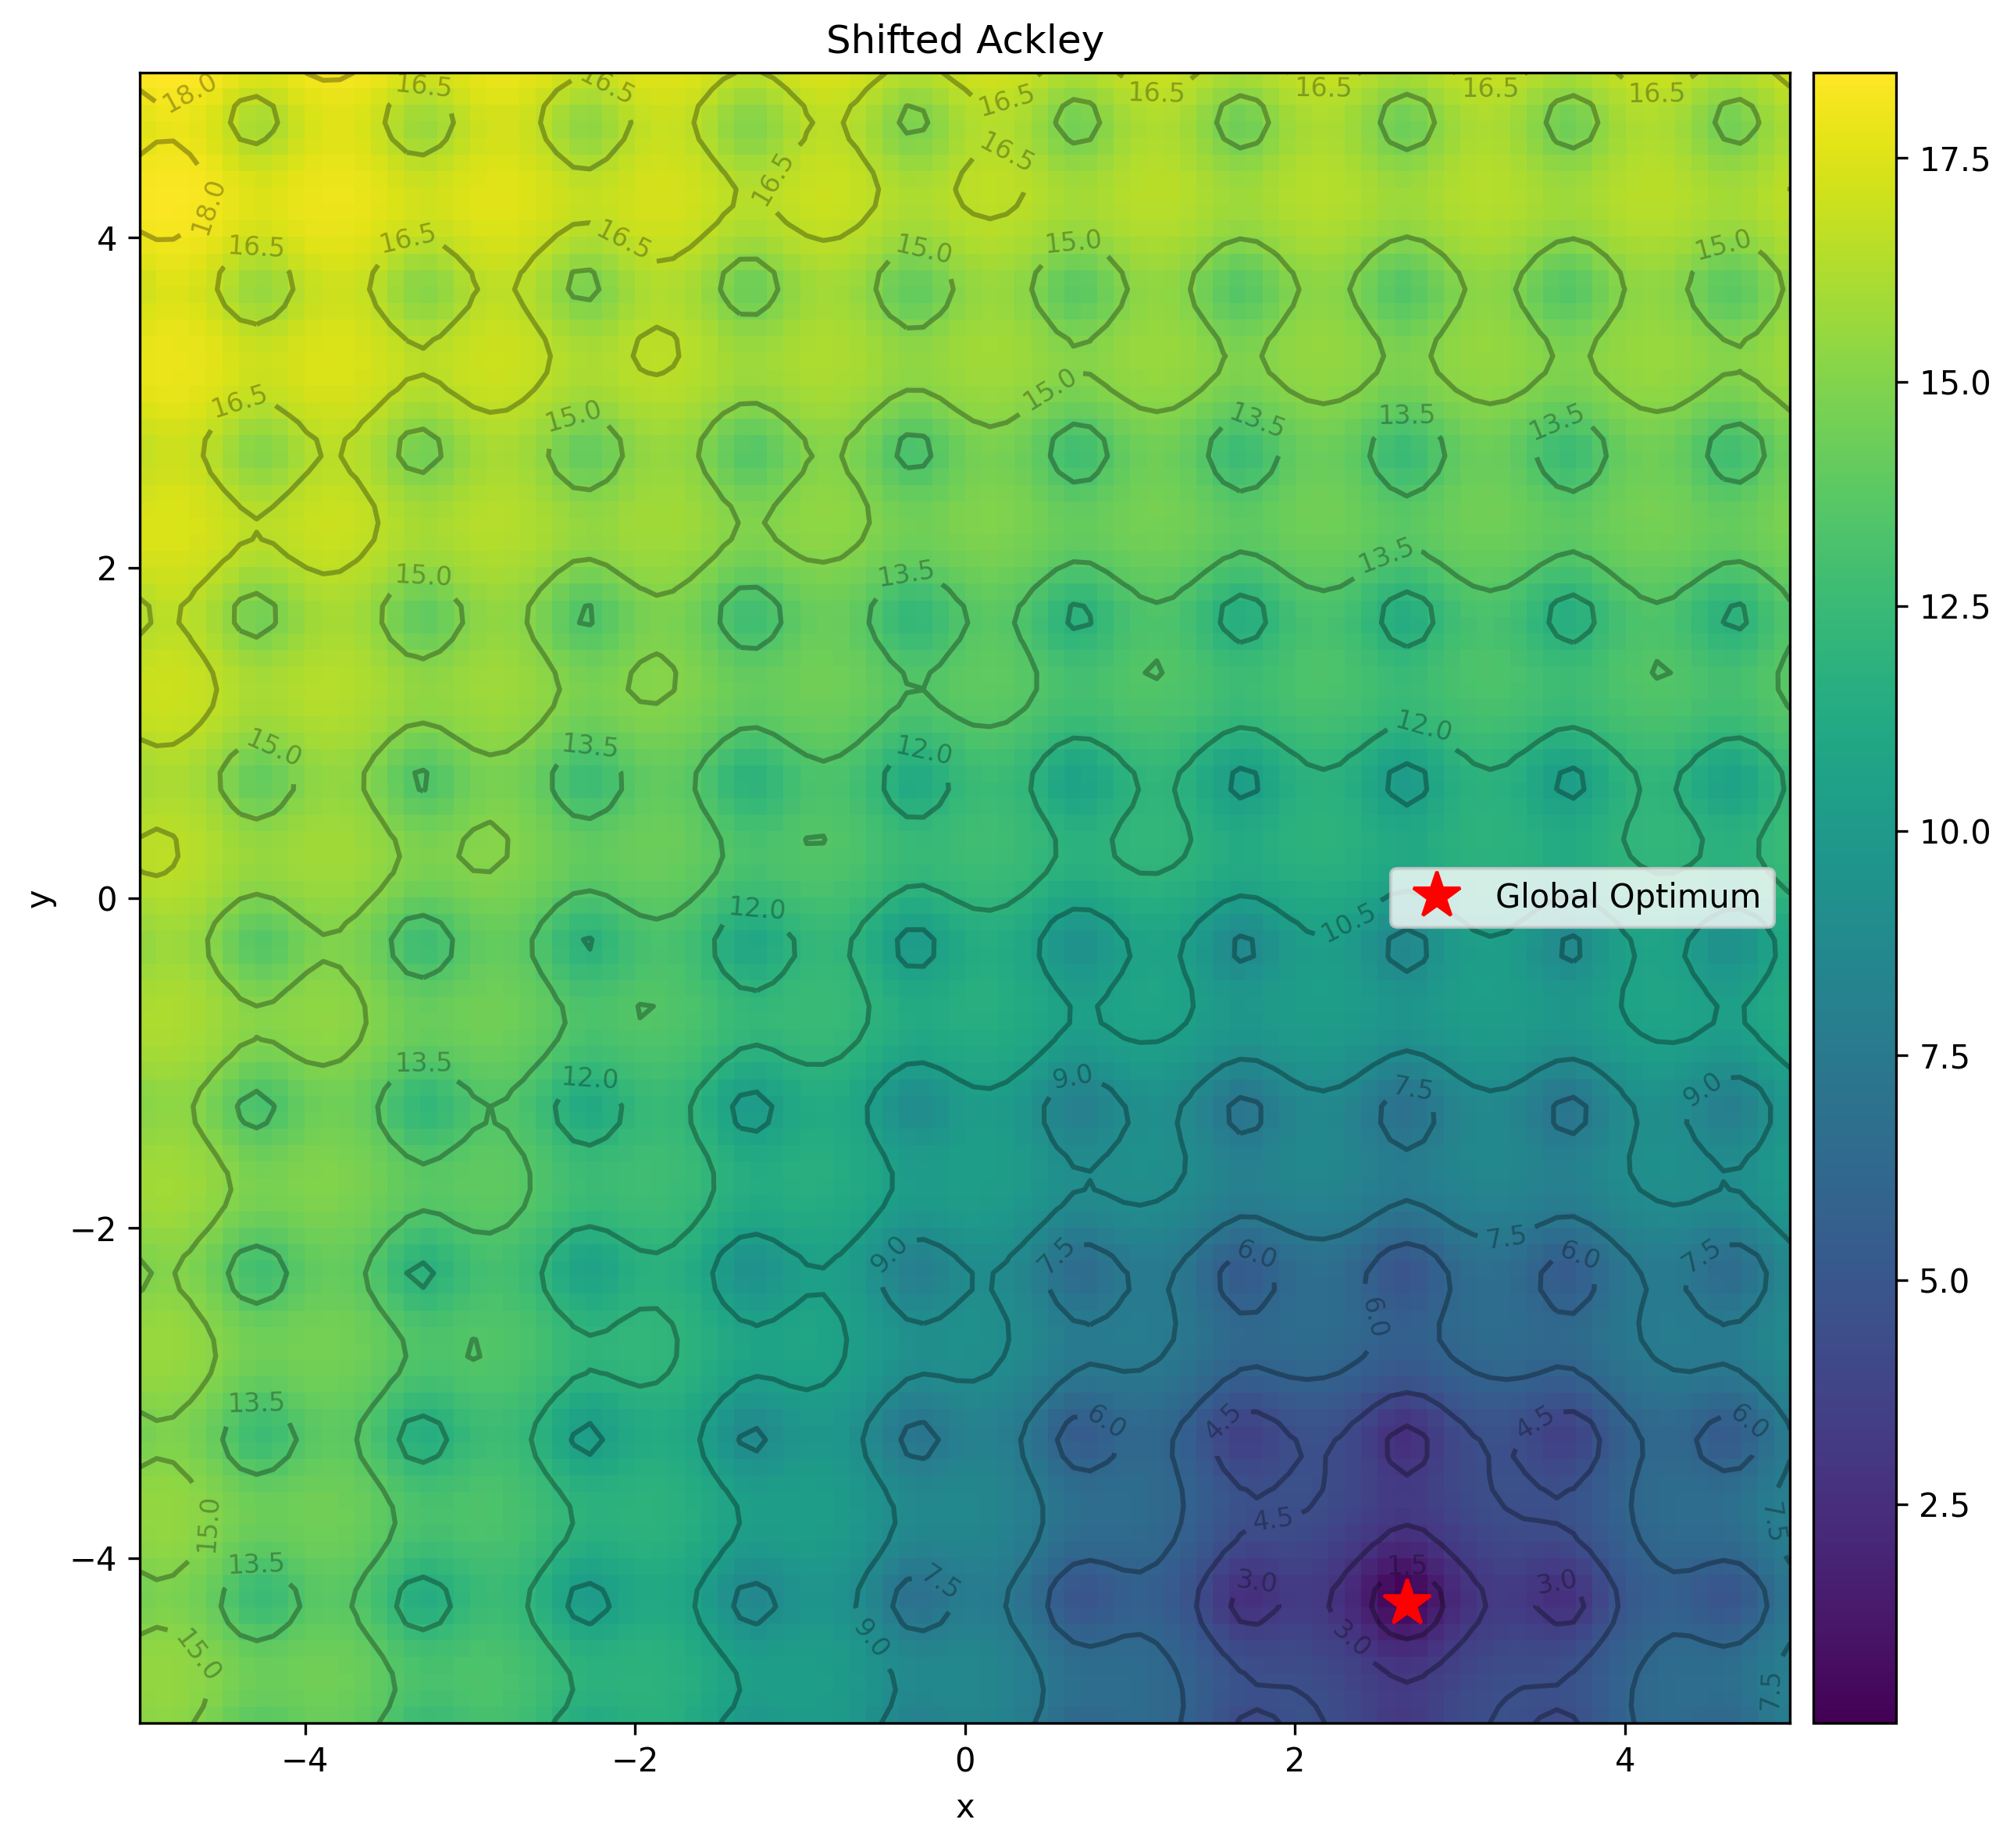
\includegraphics[width=\textwidth]{shifted_ackley.png}
    \caption{Wykres funkcji Shifted Schwefel}
    \label{fig:plot2}
\end{figure}

\begin{figure}[H]
    \centering
    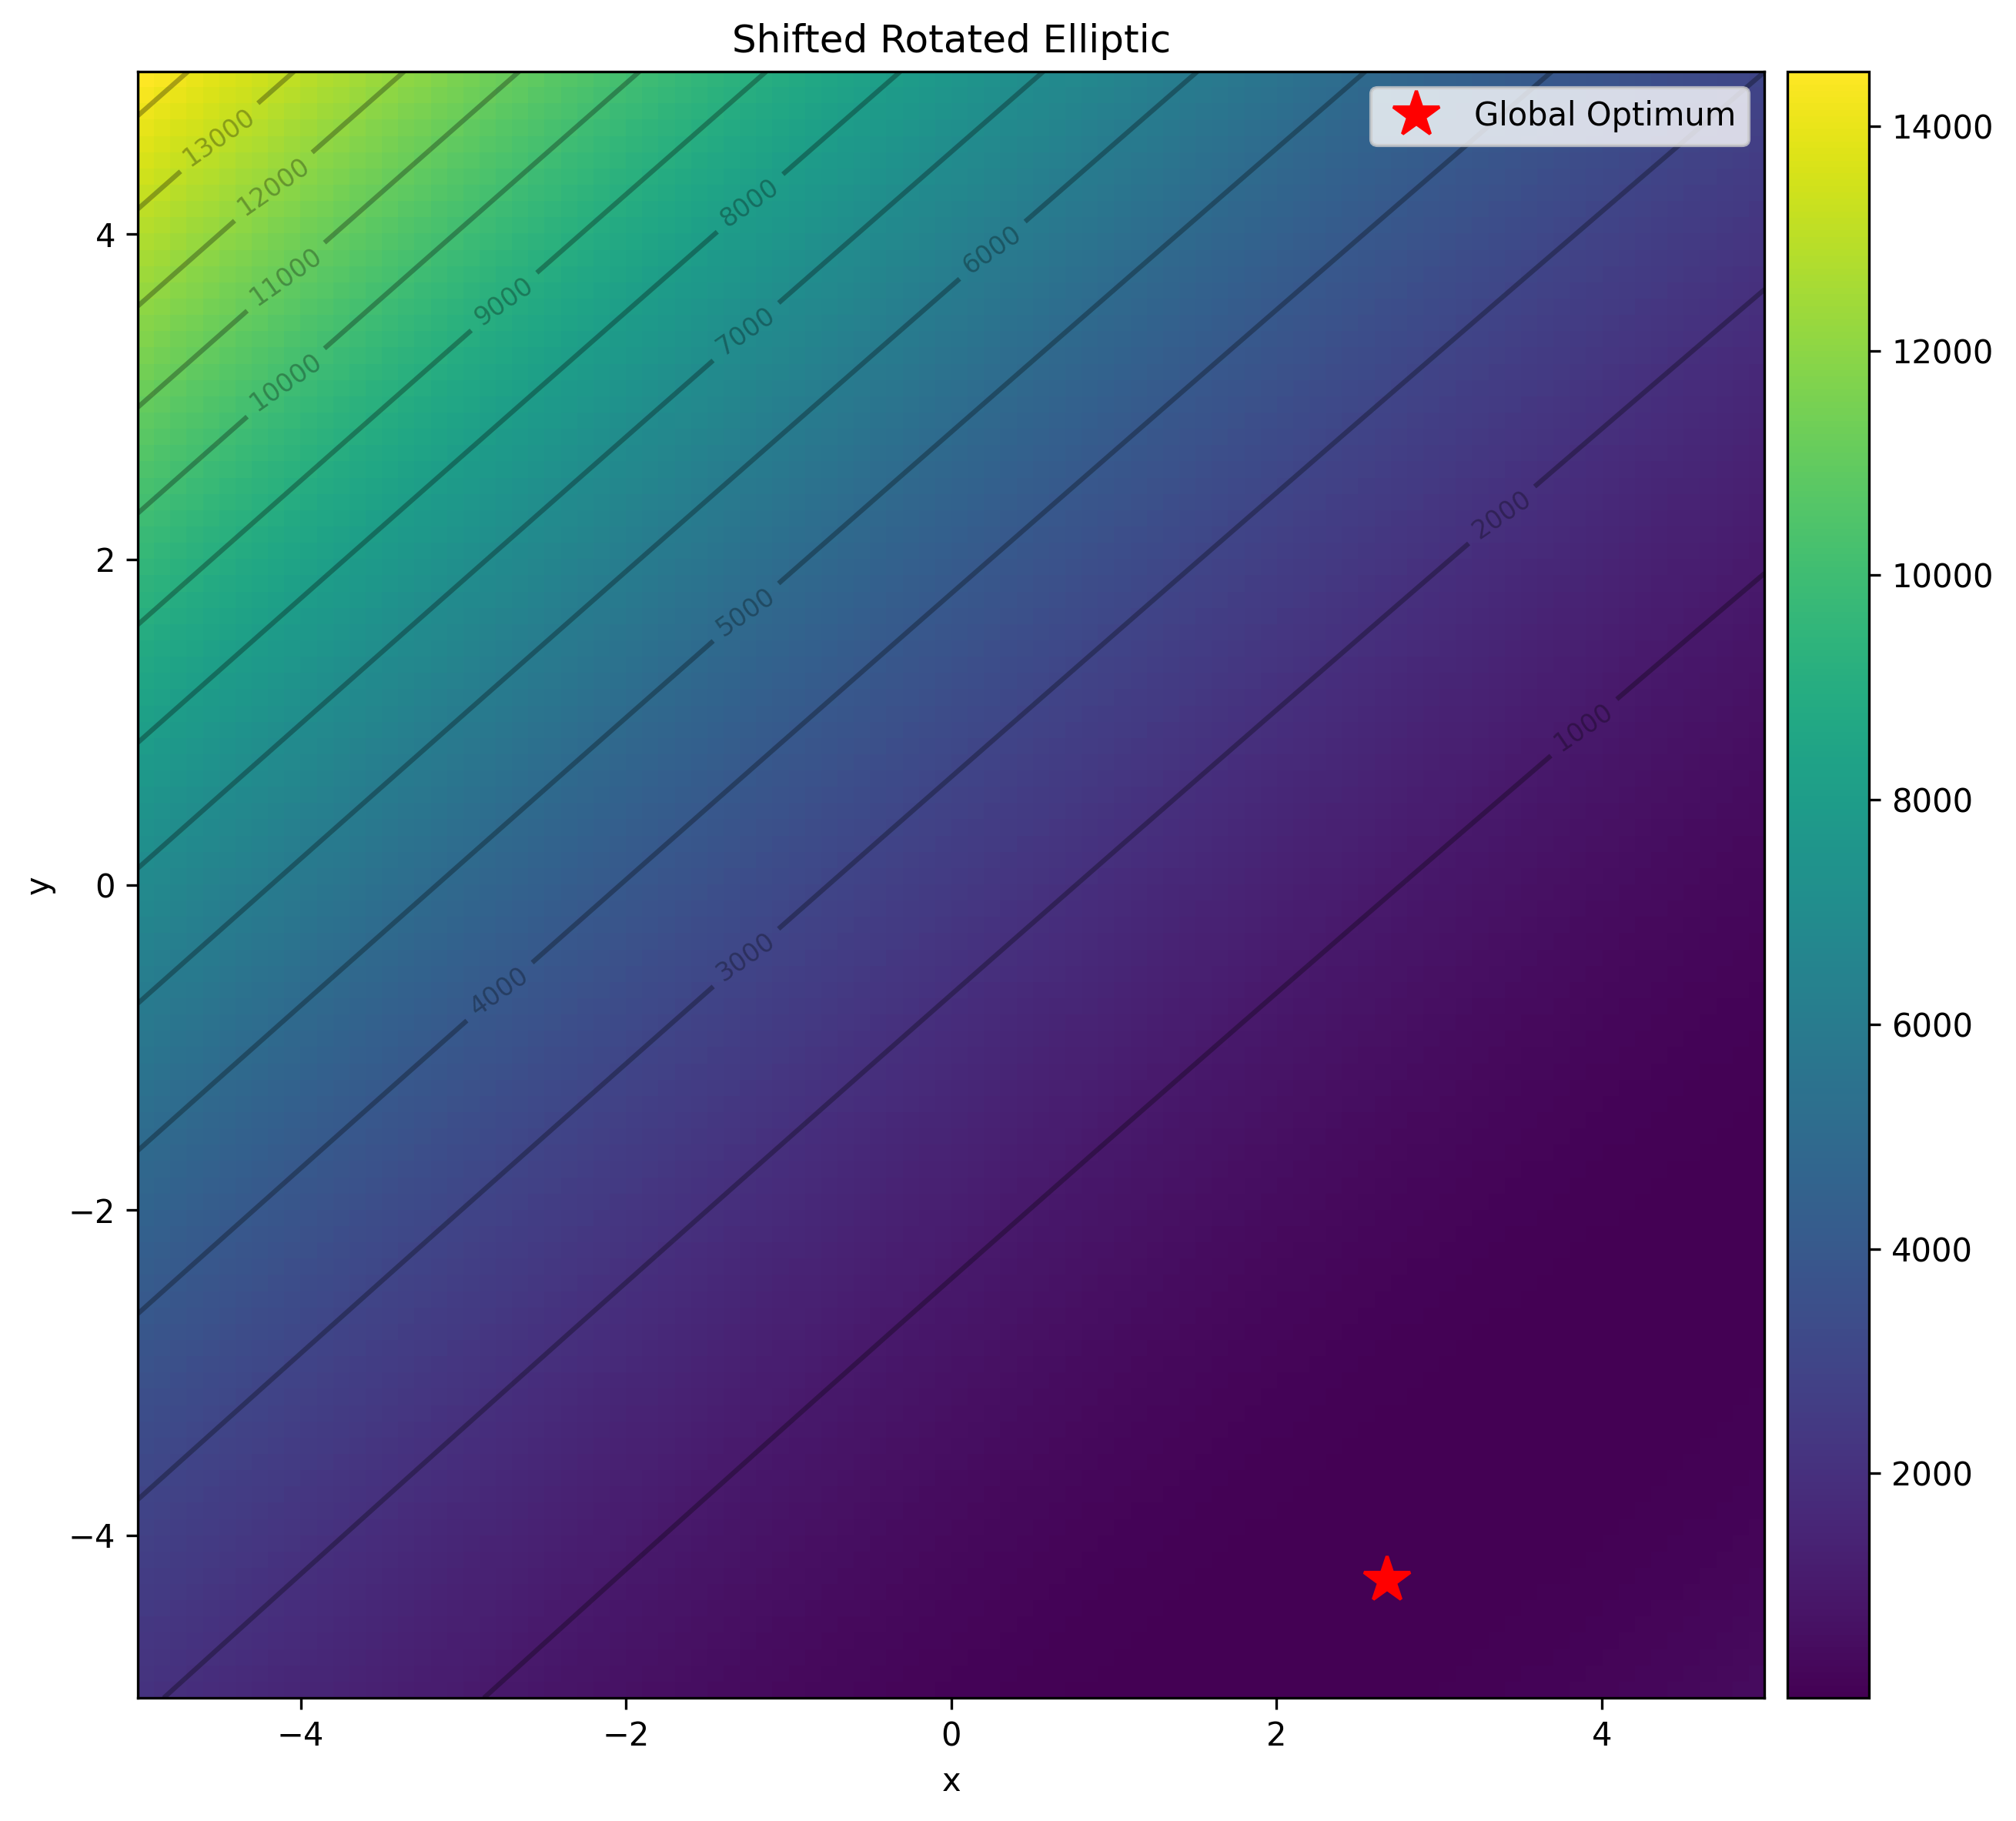
\includegraphics[width=\textwidth]{shifted_rotated_elliptic.png}
    \caption{Wykres funkcji Shifted Rotated Elliptic}
    \label{fig:plot3}
\end{figure}

\begin{figure}[H]
    \centering
    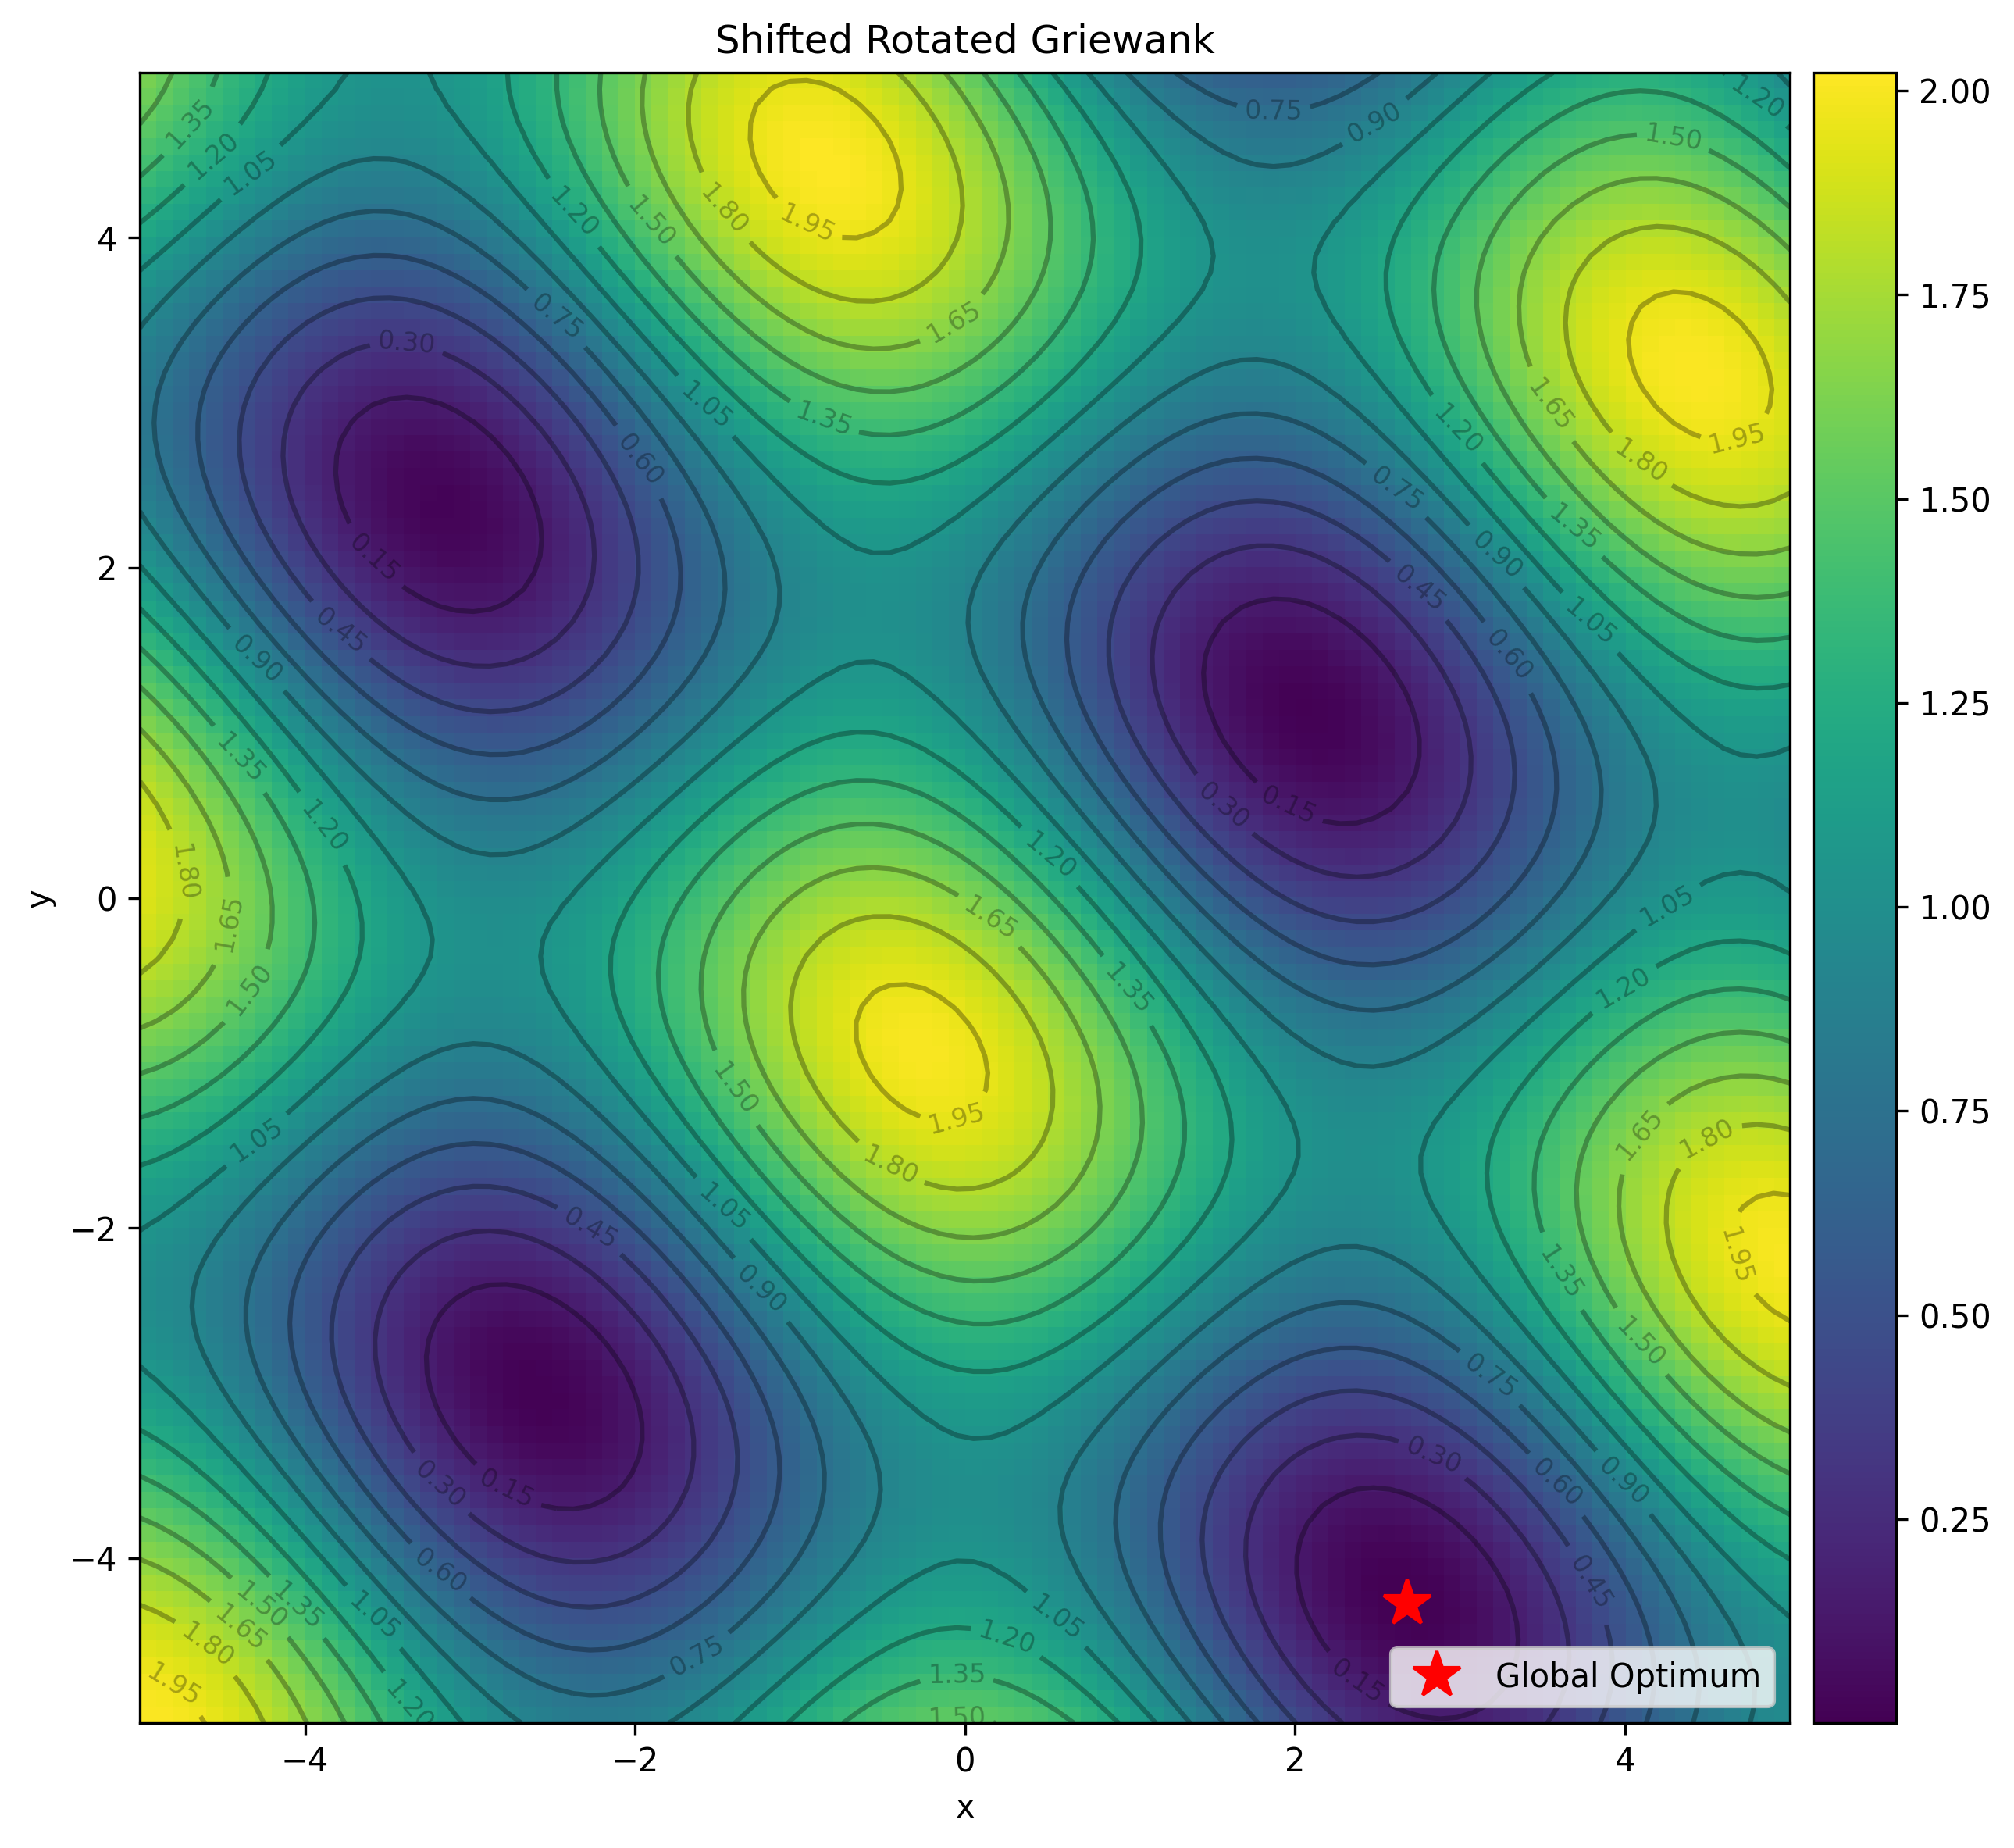
\includegraphics[width=\textwidth]{shifted_rotated_griewank.png}
    \caption{Wykres funkcji Shifted Rotated Griewank}
    \label{fig:plot4}
\end{figure}

\begin{figure}[H]
    \centering
    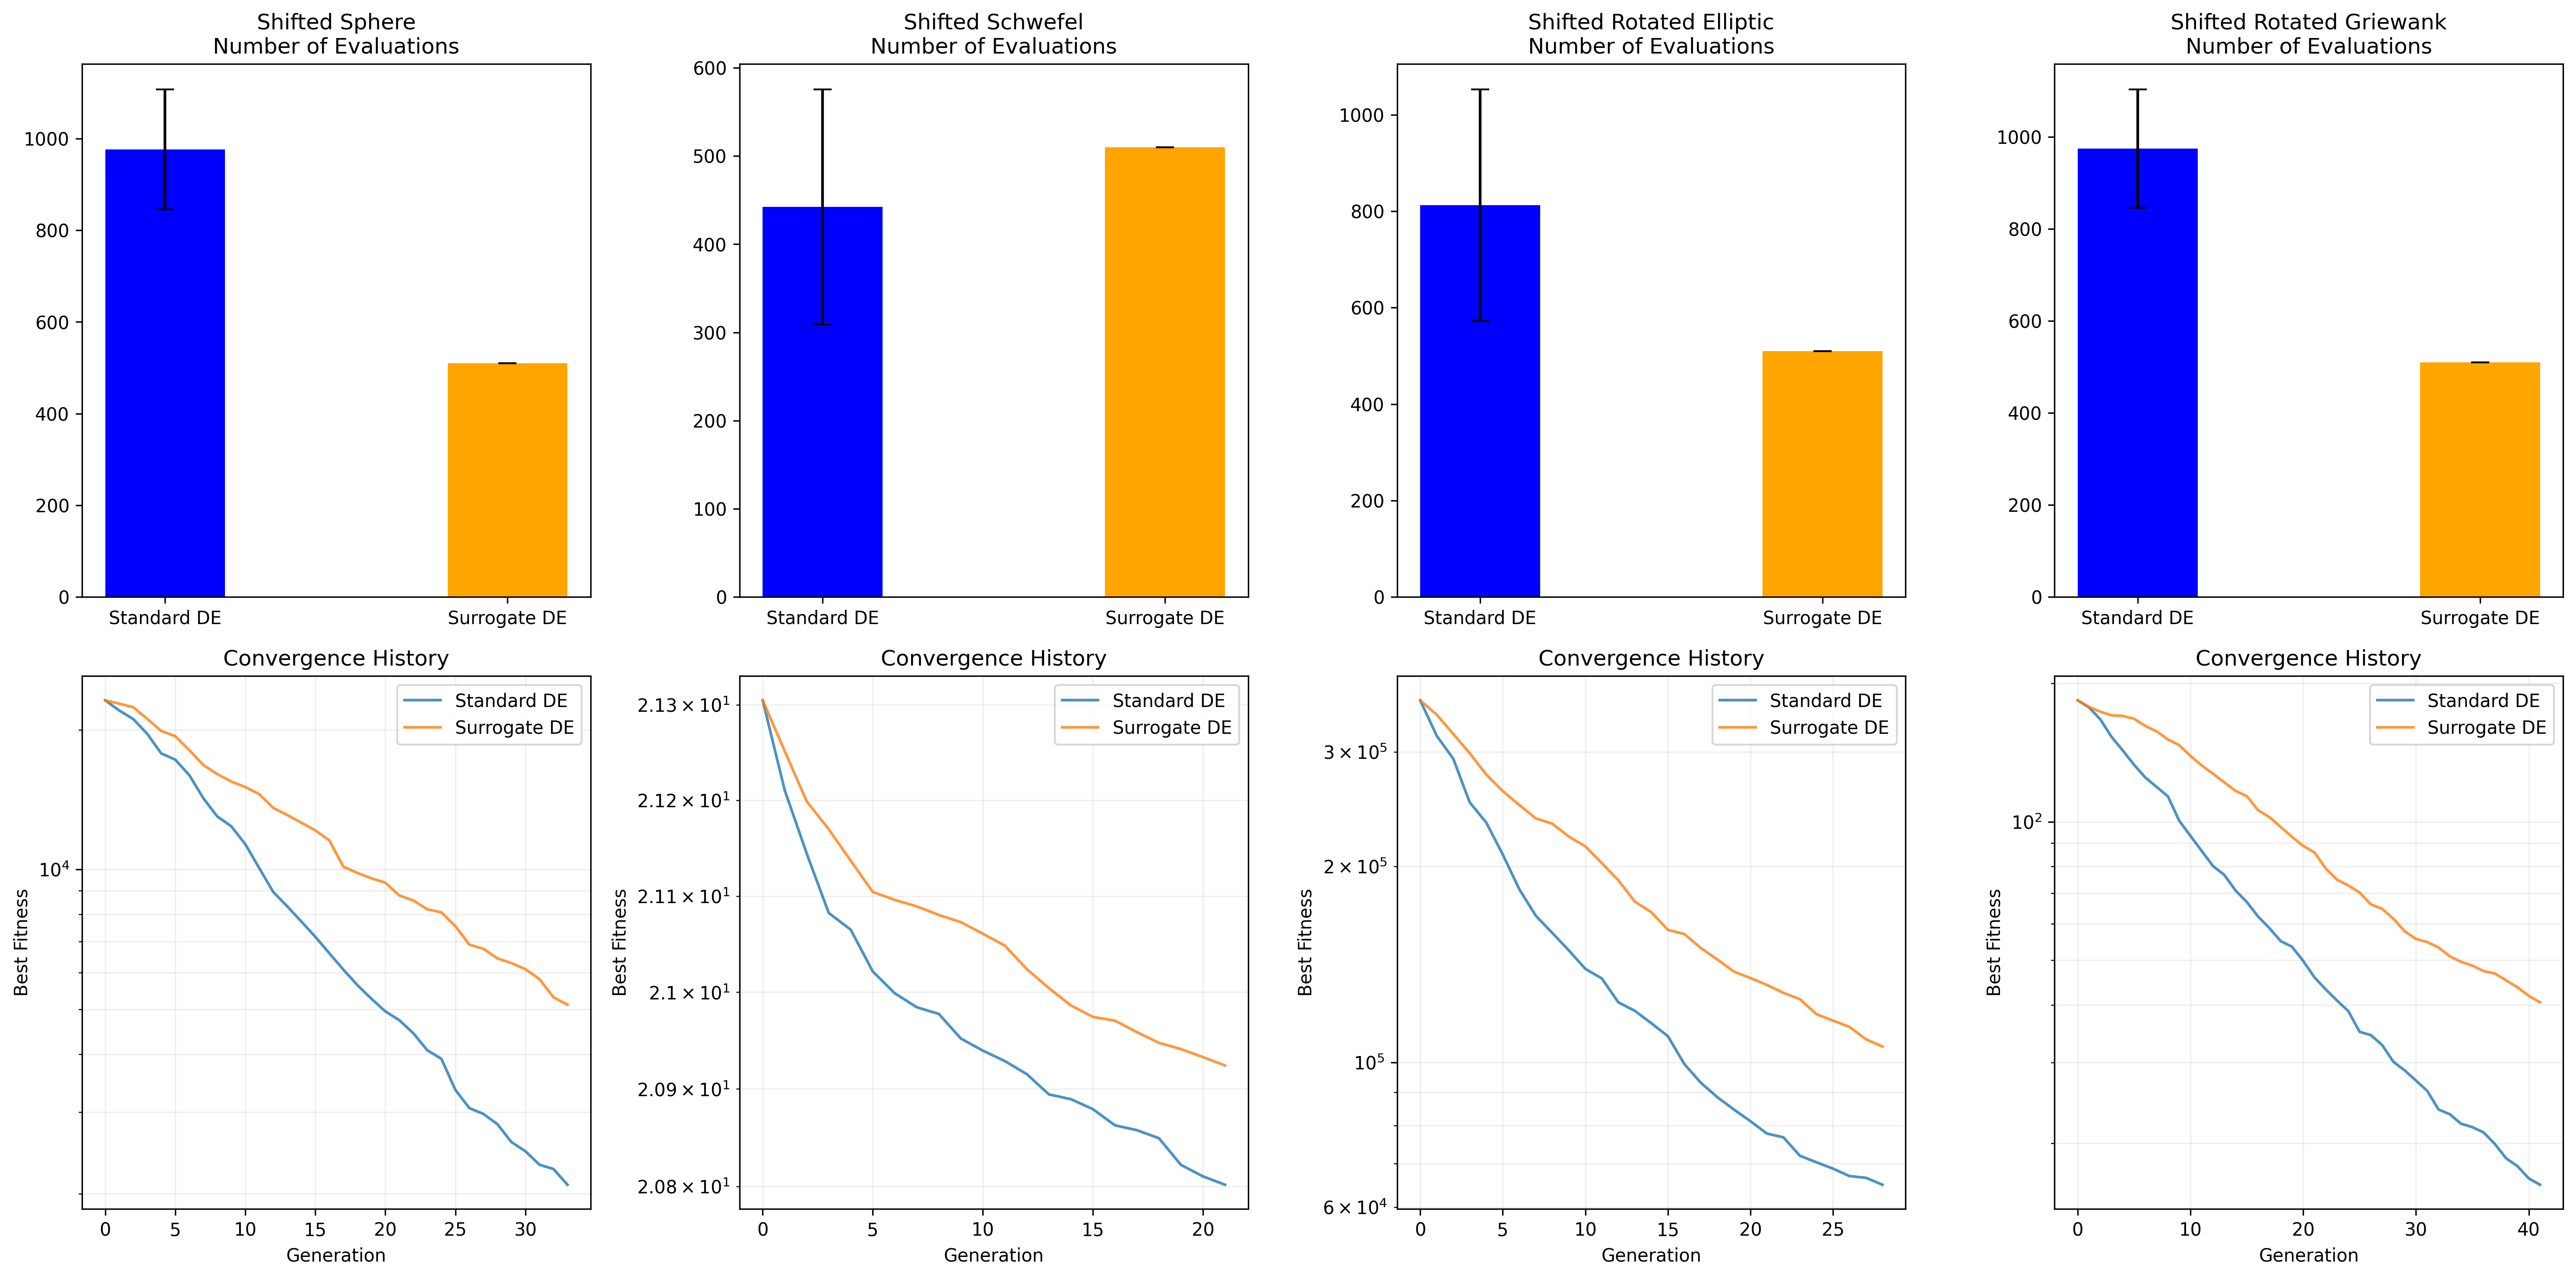
\includegraphics[width=\textwidth]{comprehensive_results.png}
    \caption{Porównanie standardowego DE z DE wykorzystującym model zastępczy}
    \label{fig:comprehensive_results}
\end{figure}

Wykresy przedstawiają wartości uśrednione po 50 powtórzeniach, dla każdej funkcji osobno. W górnym rzędzie znajduje się liczba ewaluacji wykonywanych przez algorytm ewolucji, a w dolnym najlepsze wartości w zależności od numeru generacji. 
W większości przypadków algorytm z modelem zastępczym wykonuje mniej ewaluacji funkcji celu. Jedyną funkcją, dla której otrzymaliśmy inne wyniki, była Shifted Schwefel, w przypadku której standardowa ewolucja o wiele szybciej znajdowała optymalne rozwiązanie, przez co kryterium stopu stagnacji kończyło wywoływanie algorytmu, ukracając liczbę ewaluacji. Ewolucja z modelem zastępczym z powodu wolniejszego osiągania optymalnych rozwiązań nie spełniała kryterium stagnacji. 
Na wykresach w dolnym rzędzie wyraźnie rysuje się różnica w jakości obydwu algorytmów. Algorytm z modelem zastępczym zwracał gorsze wyniki, co jest zgodne z oczekiwaniami, ponieważ model zastępczy jest tylko aproksymacją funkcji celu.

\begin{table}[H]
    \centering
    \begin{tabular}{|l|r|r|r|}
    \hline
    & \textbf{Standardowa} & \textbf{Zastępcza} & \textbf{Różnica (\%)} \\
    \hline
    \text{Shifted Sphere} & 976.40 & 510.00 & -47.77\% \\
    \hline
    \text{Shifted Schwefel} & 442.20 & 510.00 & +15.33\% \\
    \hline
    \text{Shifted Rotated Elliptic} & 812.40 & 510.00 & -37.22\% \\
    \hline
    \text{Shifted Rotated Griewank} & 974.80 & 510.00 & -47.68\% \\
    \hline
    \textbf{Średnia} & 801.45 & 510.00 & -36.37\% \\
    \hline
    \end{tabular}
    \caption{Średnia liczba ewaluacji funkcji celu}
    \label{tab:evaluations}
\end{table}

\begin{table}[H]
    \centering
    \begin{tabular}{|l|r|r|r|}
    \hline
    & \textbf{Standardowa} & \textbf{Zastępcza} & \textbf{Różnica (\%)} \\
    \hline
    \text{Shifted Sphere} & 172.55 & 1246.18 & +622.17\% \\
    \hline
    \text{Shifted Schwefel} & 20.66 & 20.62 & -0.18\% \\
    \hline
    \text{Shifted Rotated Elliptic} & 22176.33 & 34553.15 & +55.81\% \\
    \hline
    \text{Shifted Rotated Griewank} & 2.59 & 12.41 & +379.10\% \\
    \hline
    \textbf{Średnia} & 5593.03 & 8958.09 & +60.17\% \\
    \hline
    \end{tabular}
    \caption{Średnia jakość najlepszego rozwiązania}
    \label{tab:fitness}
\end{table}

Przeprowadzone eksperymenty pokazały, że zastosowanie modelu zastępczego w ewolucji różnicowej pozwala na zmniejszenie liczby ewaluacji funkcji celu (dla testowanych funkcji średnio 36.37 \%). Jakość rozwiązań uzyskiwanych przez algorytm z modelem zastępczym jest średnio o 60.17\% gorsza niż w przypadku standardowej ewolucji różnicowej. W związku z tym, zastosowanie modelu zastępczego w ewolucji różnicowej może być uzasadnione jedynie w przypadku, gdy koszt obliczeń funkcji celu jest bardzo wysoki.

\section{Wprowadzone zmiany w dokumentacji}

\subsection{Zmiany w sekcji: ewolucja różnicowa}

Dodatkowa informacja o kryterium stopu stagnacji:

Polego ono na sprawdzeniu czy przez określoną liczbę iteracji nie nastąpiła poprawa najlepszego osobnika. Jeżeli taka poprawa nie nastąpiła, algorytm kończy działanie.

\subsection{Zmiany w sekcji: wyznaczanie parametrów}

Został zmieniony sposób szukania optymalnych parametrów do testowania algorytmu. Główną zmianą było sprawdzanie z jaką skutecznością algorytm trafiał w optimum globalne zamiast sprawdzania średniej jakości rozwiązania.


Badanie zaczęliśmy od wyznaczania optymalnych parametrów ewolucji różnicowej. W tym celu przeprowadziliśmy eksperymenty dla funkcji Shifted Rotated Griewank z benchmarku CEC o 2 wymiarach. Wyznaczanie optymalnych parametrów algorytmu ewolucji różnicowej rozpoczęliśmy od wybrania domyślnych wartości wszystkich testowanych parametrów, które wydawały nam się sensowne. Dla tych wartości rozpoczęliśmy testowanie pojedynczych parametrów aby uzyskać przedziały wartości, które dają najlepsze wyniki. Dla najlepszych znalezionych przedziałów wartości przeprowadzaliśmyk kolejne testy, które ostatecznie pozwoliły nam na wybranie optymalnych wartości parametrów do dalszych testów. Procent sukcesu, na podstawie którego sprawdzaliśmy jakość parametrów był uśredniany po 50 iteracjach. 

\begin{figure}[H]
    \centering
    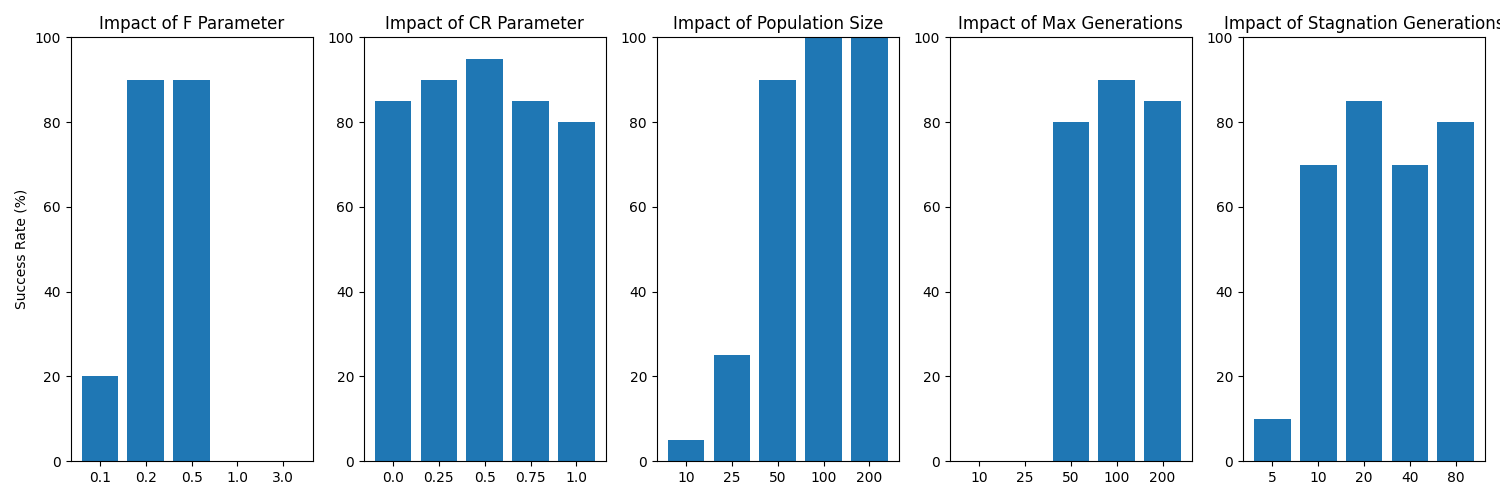
\includegraphics[width=\textwidth]{parameter_tuning_results_separate1.png}
    \caption{Wpływ parametrów na jakość algorytmu dla następujących wartości domyślnych: F = 0.5, CR = 0.5, wielkość populacji = 50, maksymalna liczba generacji = 100, stagnacja = 10}
    \label{fig:parameter_results1}
\end{figure}

\begin{figure}[H]
    \centering
    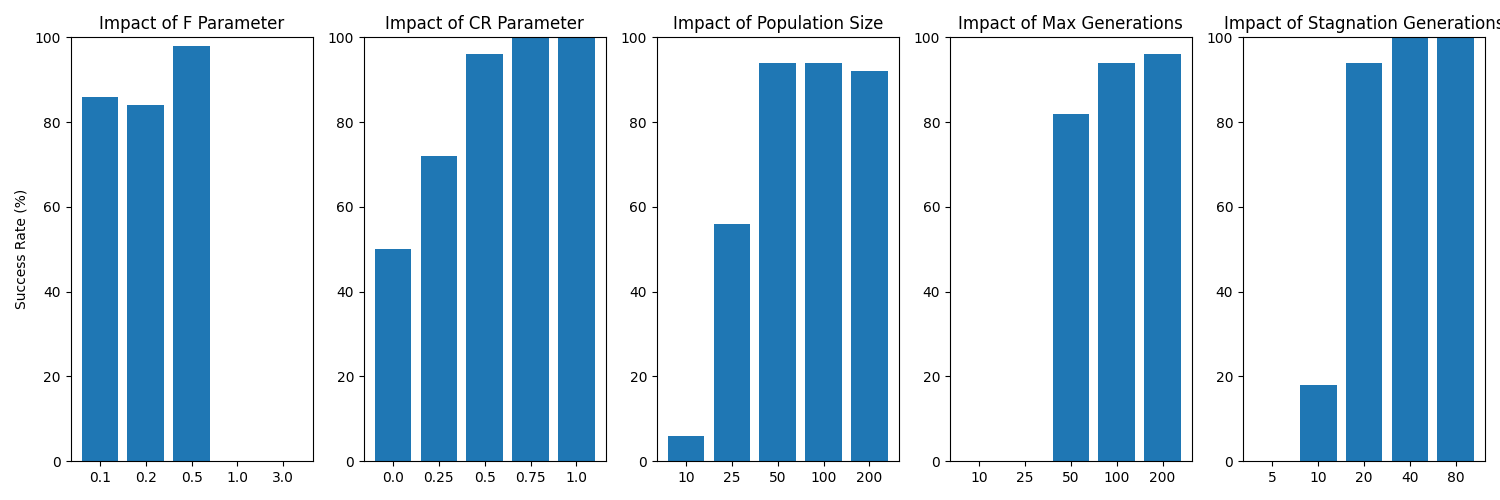
\includegraphics[width=\textwidth]{parameter_tuning_results_separate2.png}
    \caption{Wpływ parametrów na jakość algorytmu dla następujących wartości domyślnych: F = 0.5, CR = 0.5, wielkość populacji = 100, maksymalna liczba generacji = 100, stagnacja = 10}
    \label{fig:parameter_results2}
\end{figure}

\begin{figure}[H]
    \centering
    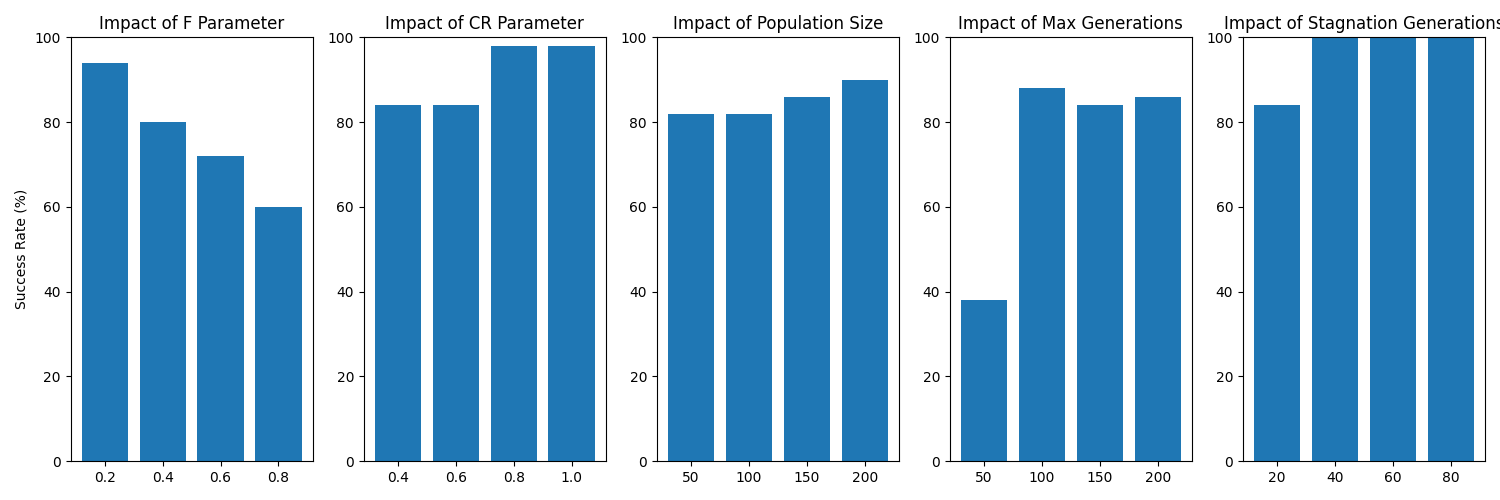
\includegraphics[width=\textwidth]{parameter_tuning_results_separate3.png}
    \caption{Wpływ parametrów na jakość algorytmu dla następujących wartości domyślnych: F = 0.5, CR = 0.5, wielkość populacji = 200, maksymalna liczba generacji = 100, stagnacja = 20}
    \label{fig:parameter_results3}
\end{figure}

\begin{figure}[H]
    \centering
    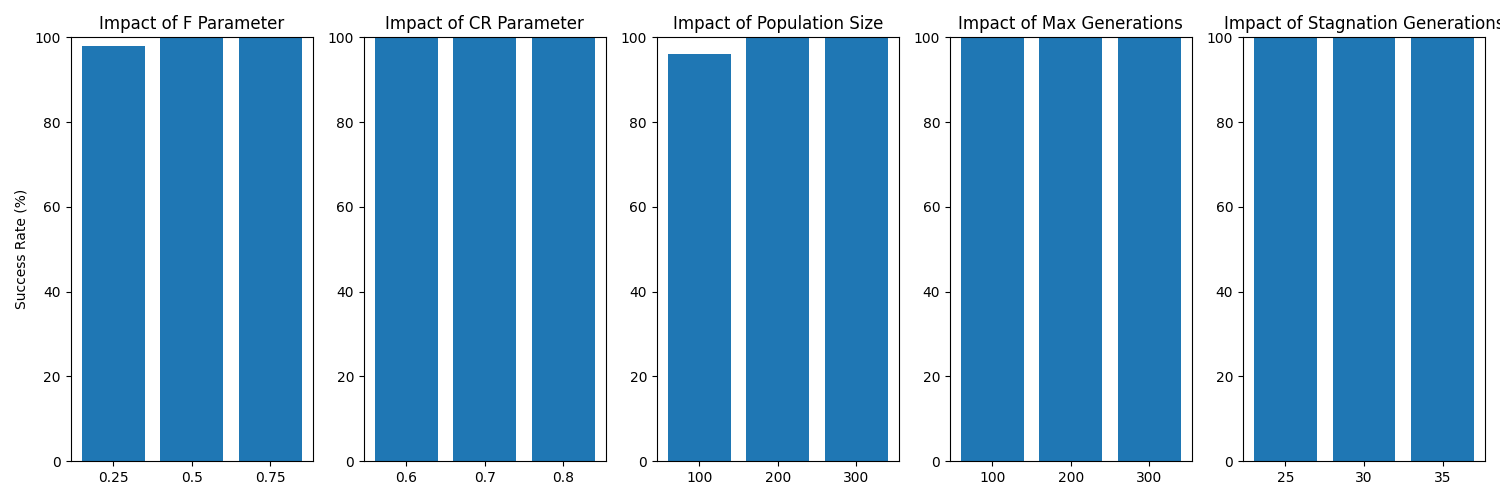
\includegraphics[width=\textwidth]{parameter_tuning_results_separate4.png}
    \caption{Wpływ parametrów na jakość algorytmu dla następujących wartości domyślnych: F = 0.5, CR = 0.8, wielkość populacji = 200, maksymalna liczba generacji = 100, stagnacja = 40}
    \label{fig:parameter_results4}
\end{figure}

Na podstawie przeprowadzonych eksperymentów wyznaczyliśmy optymalne wartości parametrów algorytmu ewolucji różnicowej:
\begin{enumerate}
    \item F - 0.5
    \item CR - 0.7
    \item Wielkość populacji - 200
    \item Maksymalna liczba generacji - 300
    \item Stagnacja - 30
\end{enumerate}

\subsection{Zmiany w sekcji: wyznaczanie parametrów drzewa regresyjnego}

Sekcja ta została całkowicie przerobiona aby lepiej przedstawić proces wyznaczania optymalnych parametrów drzewa regresyjnego.

Aby wyznaczyć optymalne parametry drzewa regresyjnego, algorytm uruchomiliśmy dla dwuwymiarowej wersji funkcji Shifted Rotated Griewank z benchmarku CEC. Wyznaczyliśmy parametry drzewa regresyjnego w ten sam sposób, co parametry ewolucji różnicowej - poprzez testowanie pojedynczych parametrów dla domyślnych wartości pozostałych parametrów.

\begin{figure}[H]
    \centering
    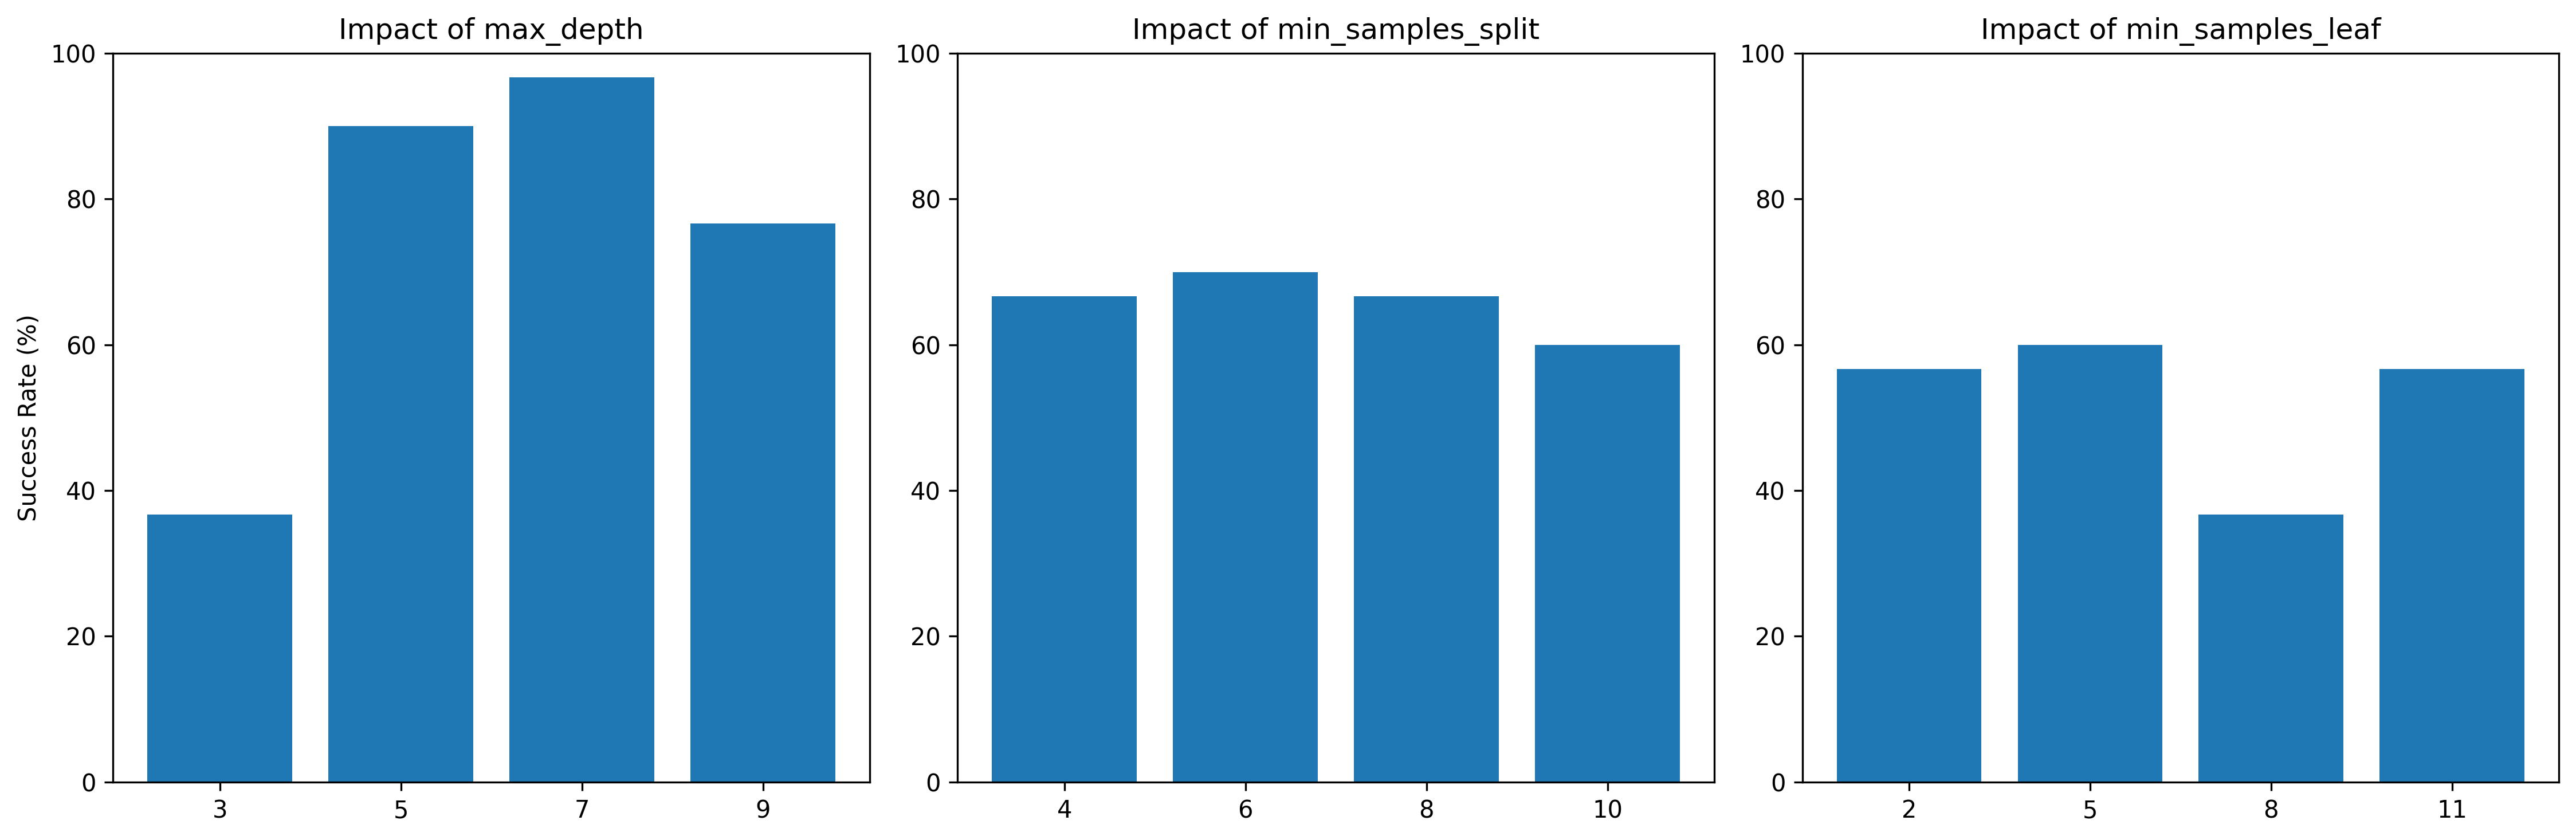
\includegraphics[width=\textwidth]{tree_parameter_tuning_separate_results2.png}
    \caption{Wpływ parametrów drzewa regresyjnego na skuteczność działania algorytmu dla następujących wartości domyślnych: maksymalna głębokość = 10, minimalna liczba próbek do podziału = 1, minimalna liczba próbek w liściu = 3}
    \label{fig:tree_parameter_results1}
\end{figure}

\begin{figure}[H]
    \centering
    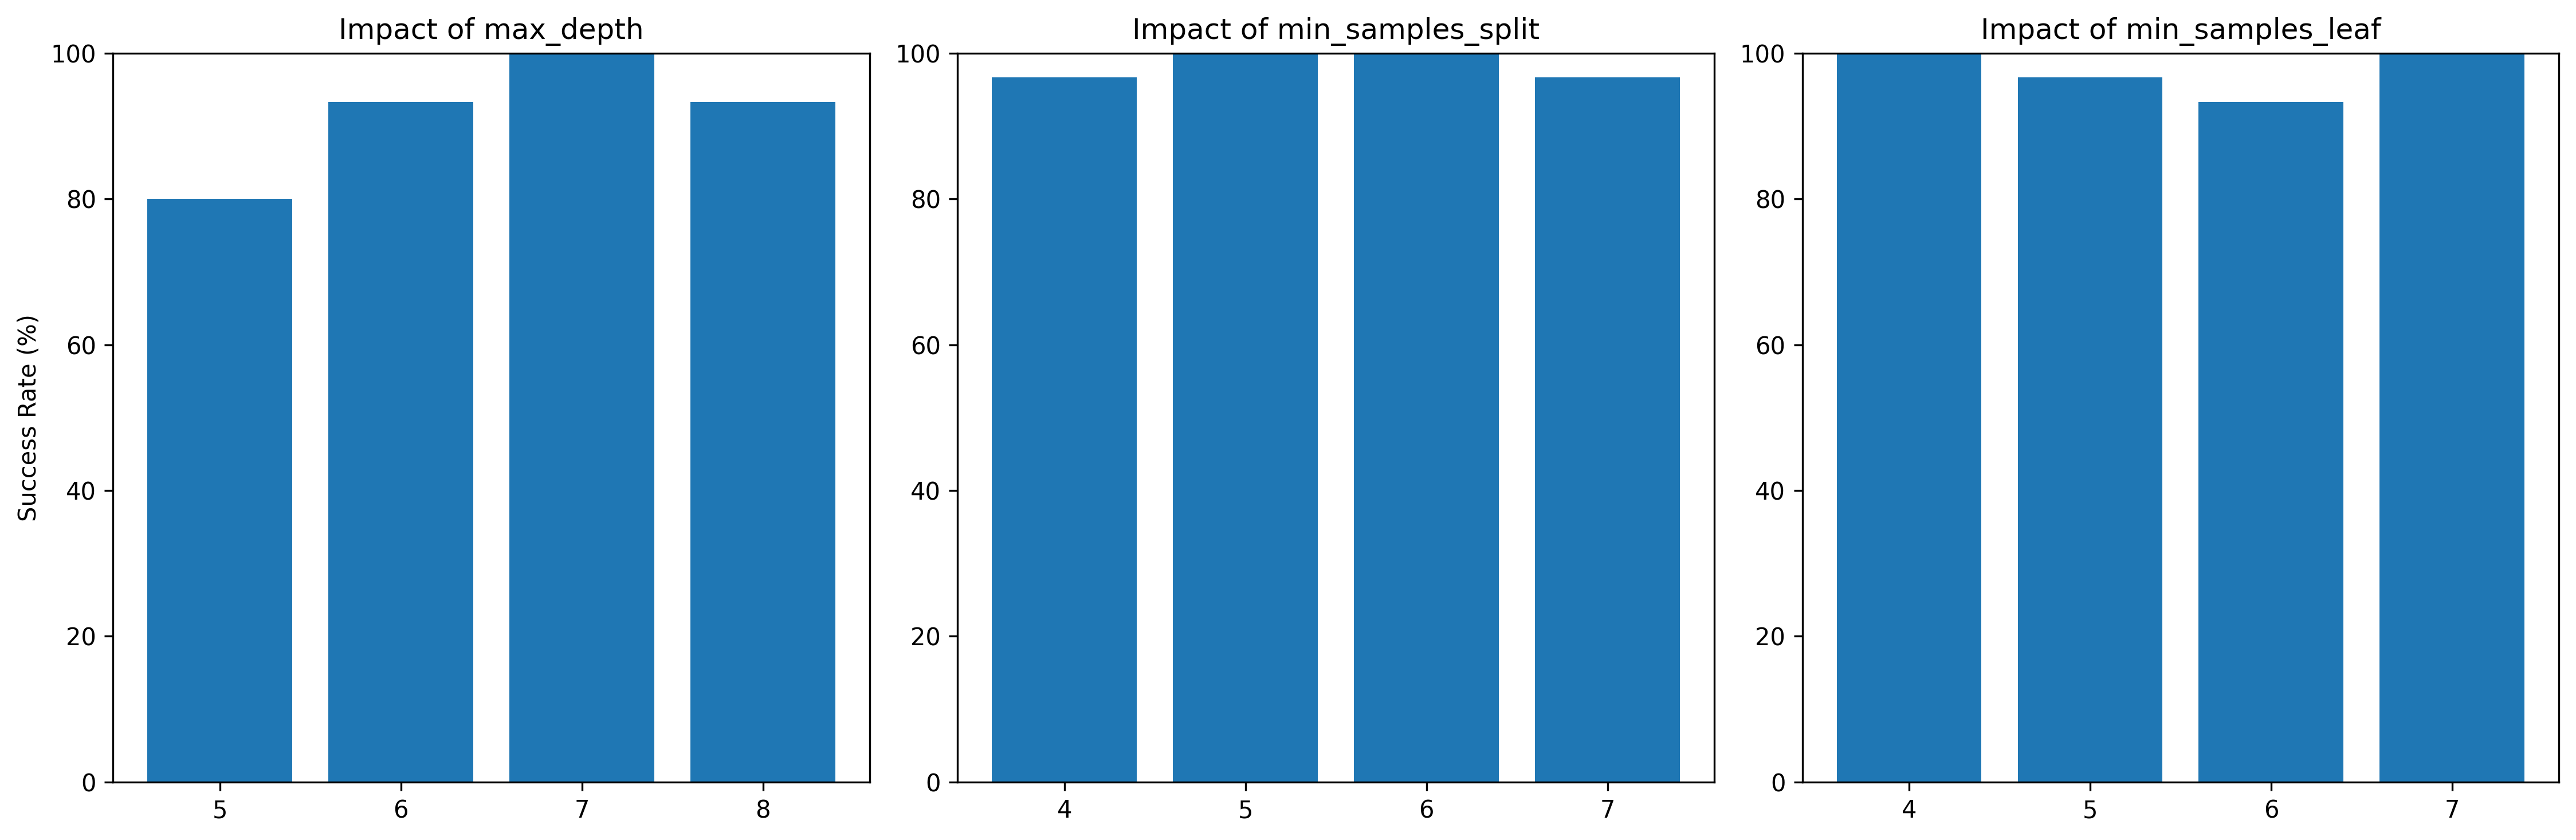
\includegraphics[width=\textwidth]{tree_parameter_tuning_separate_results3.png}
    \caption{Wpływ parametrów drzewa regresyjnego na skuteczność działania algorytmu dla następujących wartości domyślnych: maksymalna głębokość = 7, minimalna liczba próbek do podziału = 5, minimalna liczba próbek w liściu = 4}
    \label{fig:tree_parameter_results2}
\end{figure}

Na podstawie przeprowadzonych eksperymentów udało nam się wyznaczyć optymalne parametry drzewa regresyjnego:

\begin{enumerate}
    \item Maksymalna głębokość - 7
    \item Minimalna liczba próbek do podziału - 5
    \item Minimalna liczba próbek w liściu - 4
\end{enumerate}

Ostatnie dwa parametry, które przetestowaliśmy w celu uzyskania jak najleszych wyników to:
\begin{enumerate}
    \item procent najlepszych rozwiązań, które będą ewaluowane
    \item częstotliwość uczenia modelu zastępczego - co ile generacji model będzie trenowany na nowych danych
\end{enumerate}

Na podstawie ekperymentów, których wyniki zostały przedstawione poniżej, udało nam się wyznaczyć optymalne wartości tych parametrów:
\begin{enumerate}
    \item procent najlepszych rozwiązań, które będą ewaluowane - 0.65
    \item częstotliwość uczenia modelu zastępczego - 16
\end{enumerate}

Dla wartości większych niż powyższe algorytm zwacał porównywalne wyniki, jednak kosztem większej ilości ewaluacji funkcji celu. Dla wartości mniejszych niż powyższe algortm zwracał gorsze wyniki.

\begin{figure}[H]
    \centering
    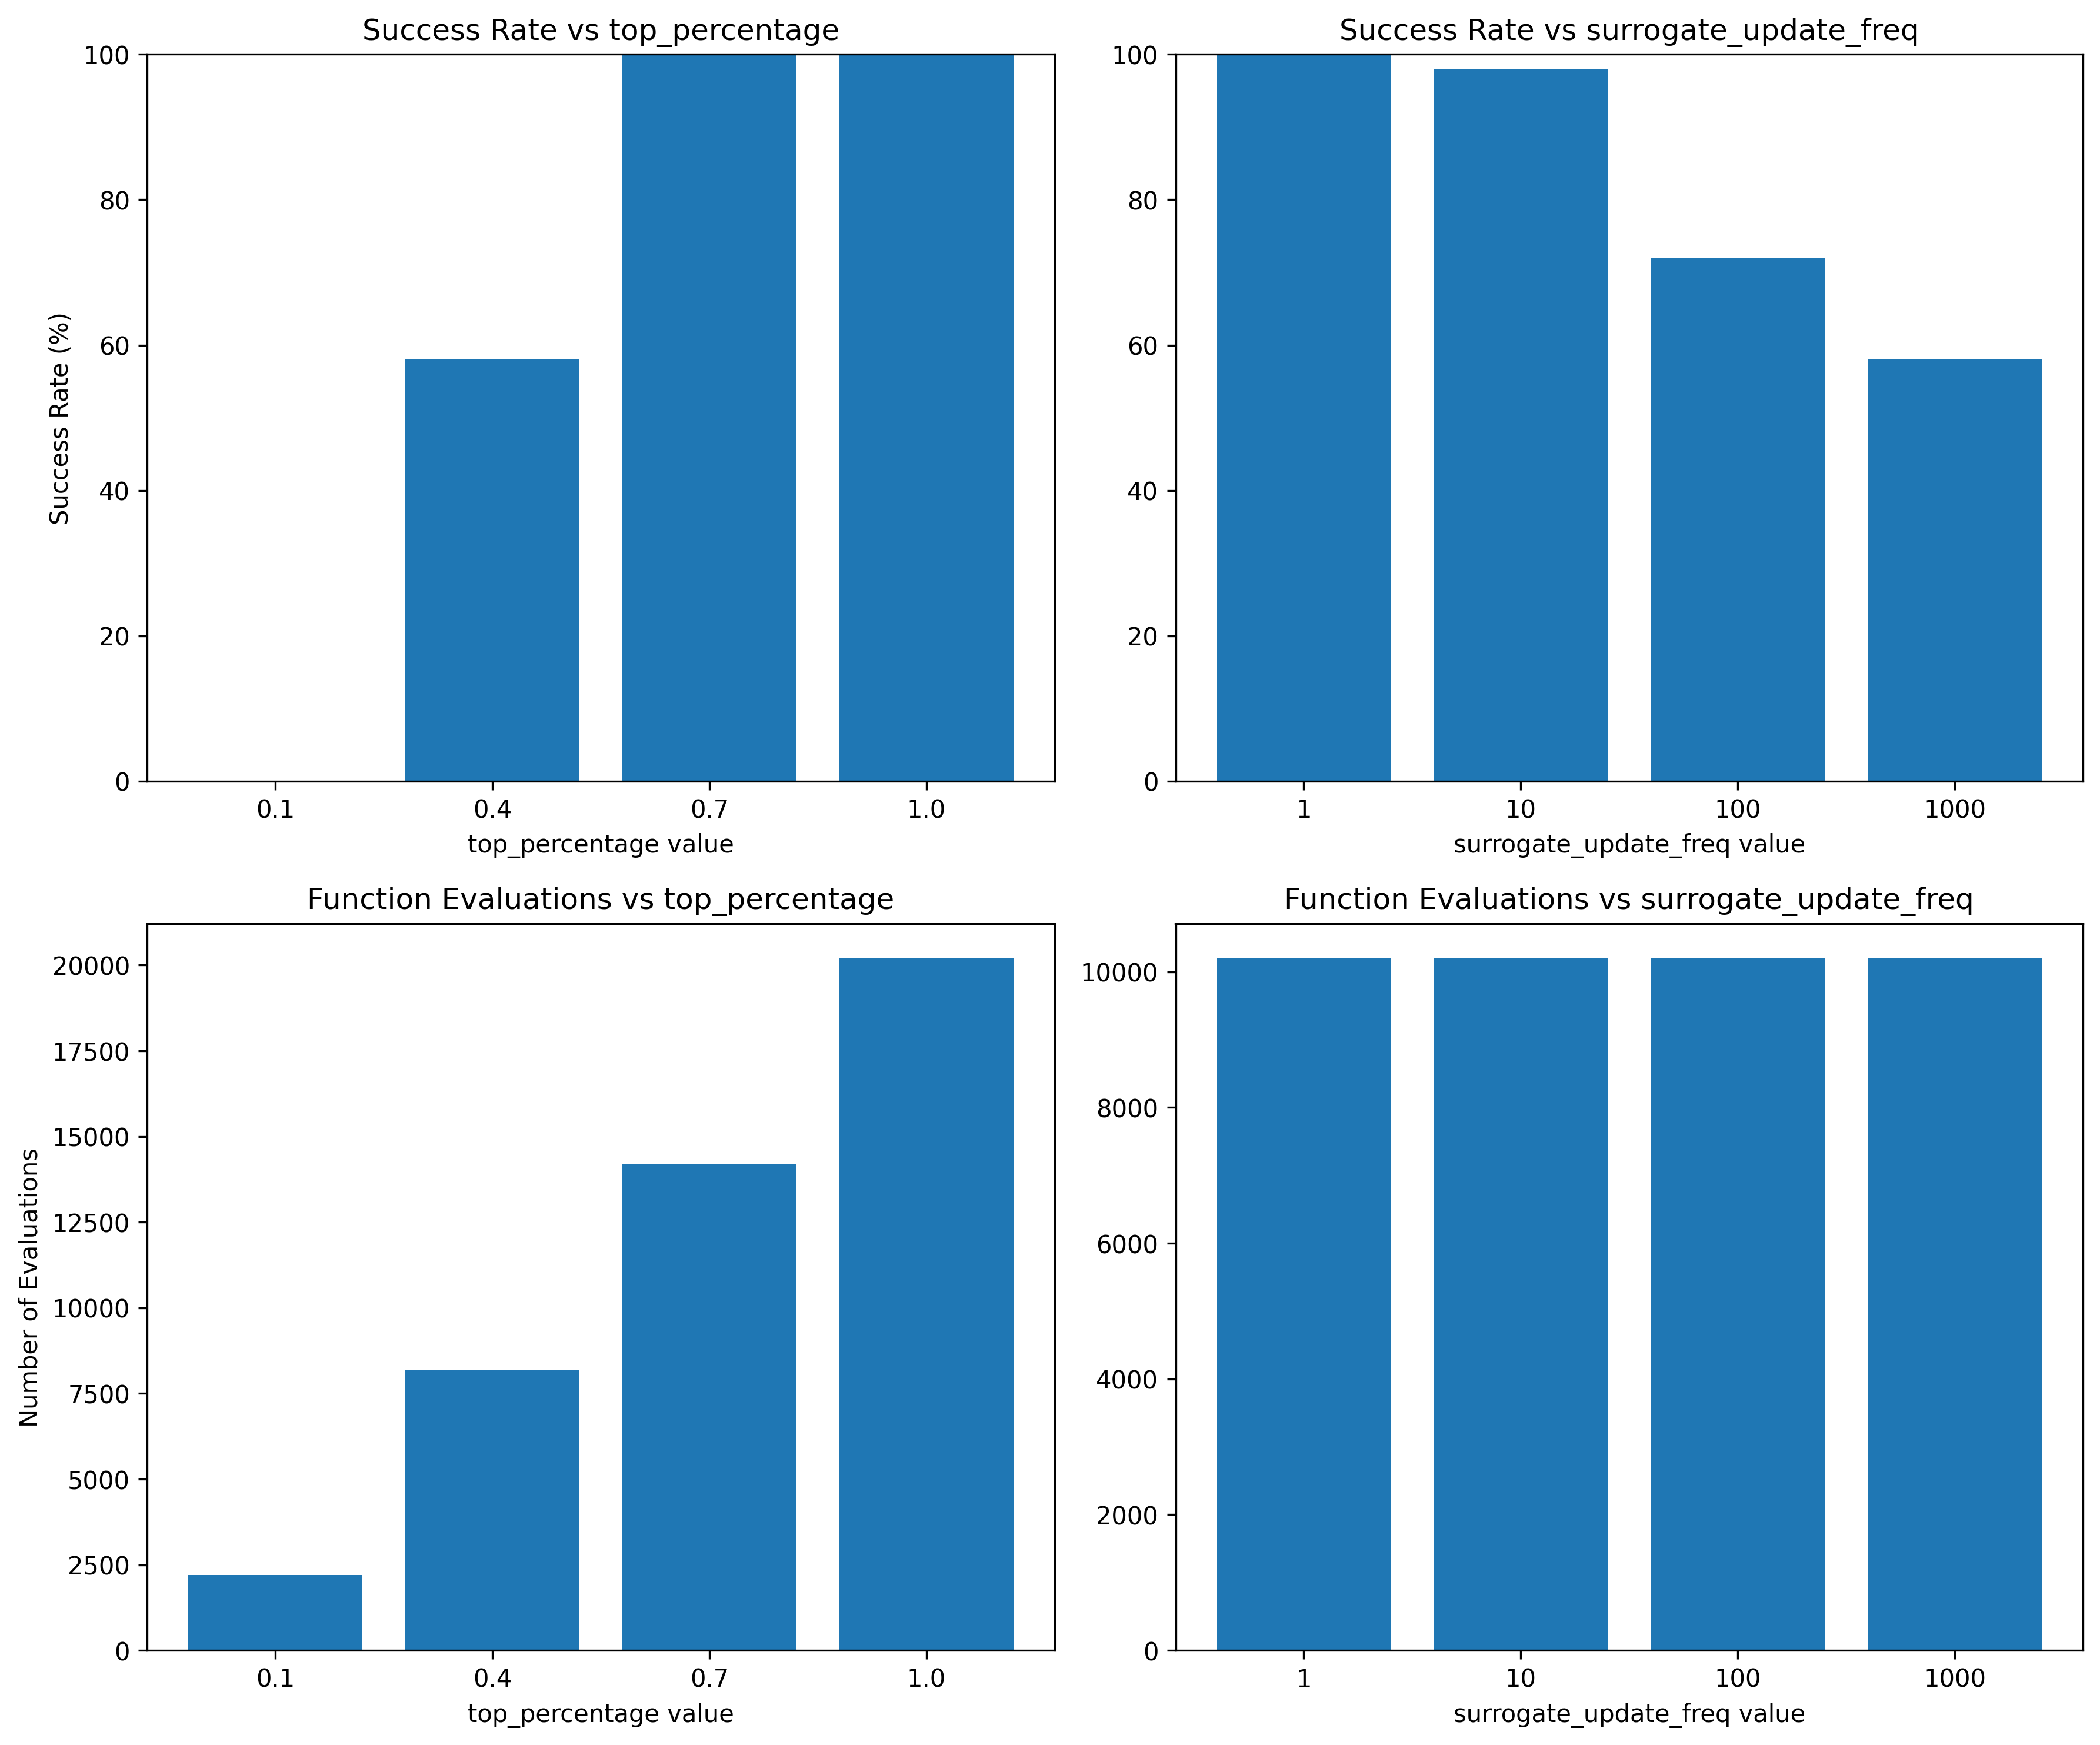
\includegraphics[width=\textwidth]{surrogate_de_parameter_tuning_results1.png}
    \caption{Wpływ procentu najlepszych rozwiązań, które są ewaluowane oraz częstotliwości uczenia modelu na skuteczność działania algorytmu dla następujących wartości domyślnych: procent najlepszych rozwiązań = 0.5, częstotliwość uczenia = 5}
    \label{fig:surogate_de_parameter_results1}
\end{figure}

\begin{figure}[H]
    \centering
    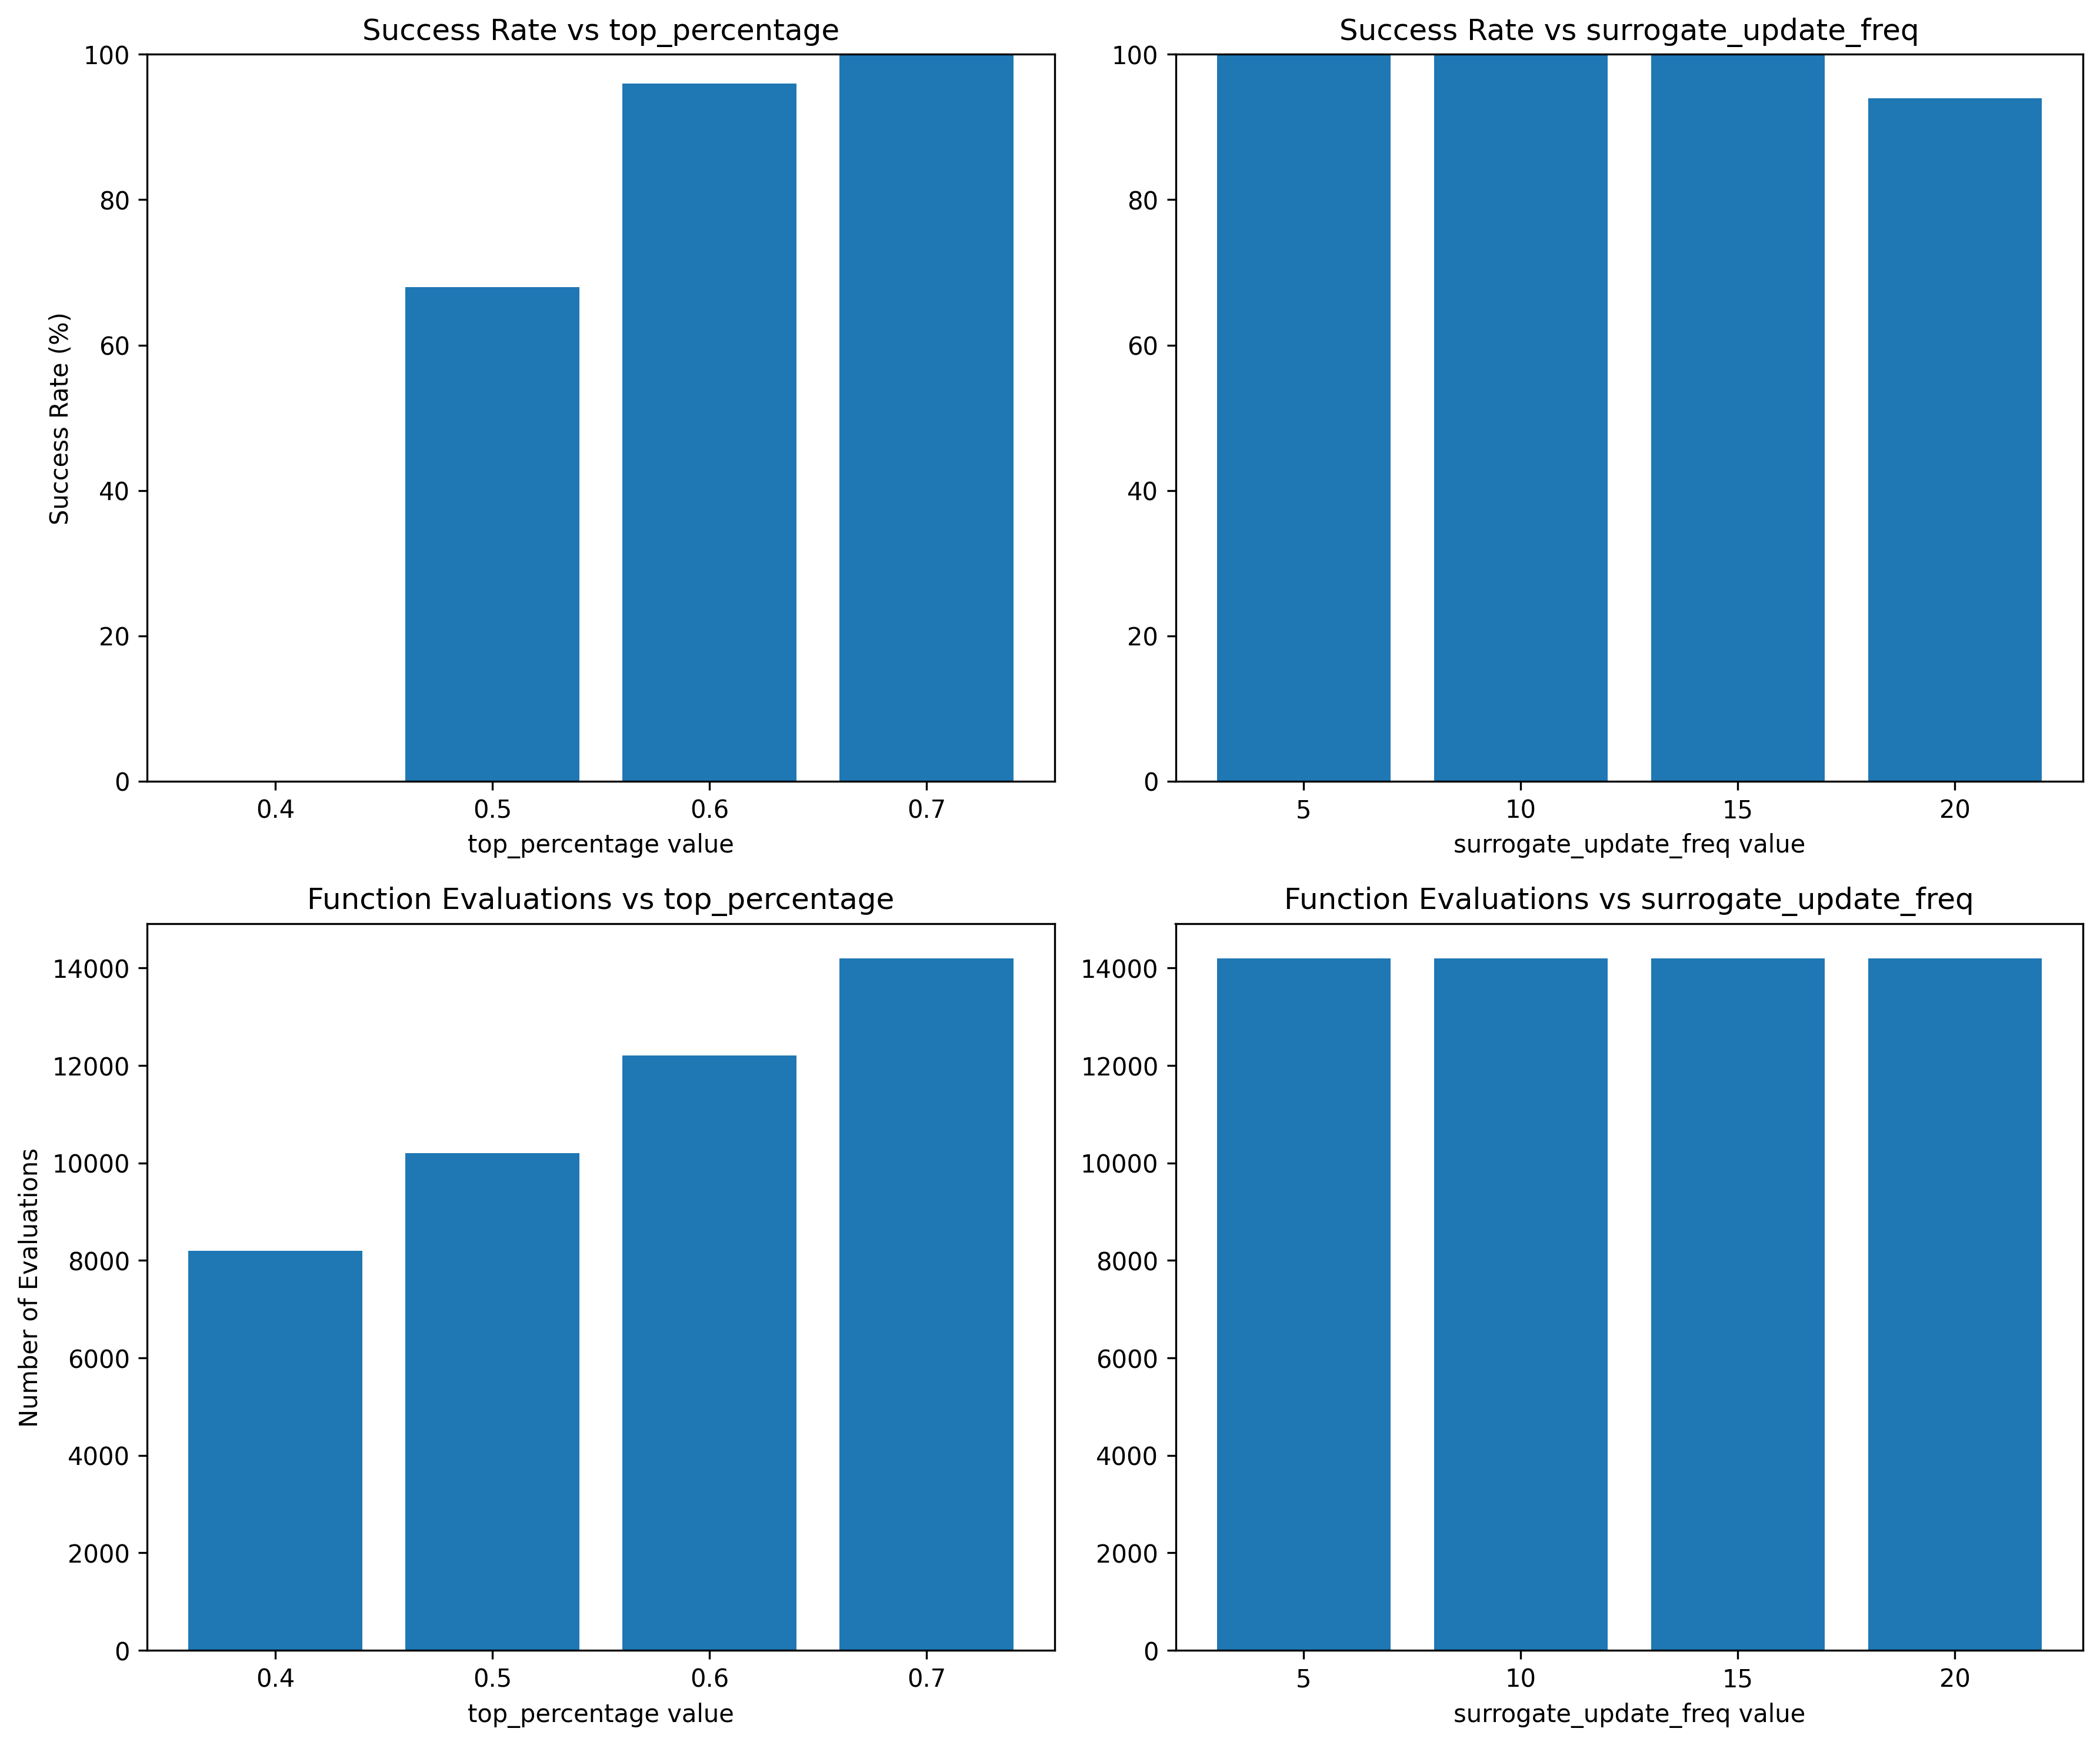
\includegraphics[width=\textwidth]{surrogate_de_parameter_tuning_results2.png}
    \caption{Wpływ procentu najlepszych rozwiązań, które są ewaluowane oraz częstotliwości uczenia modelu na skuteczność działania algorytmu dla następujących wartości domyślnych: procent najlepszych rozwiązań = 0.7, częstotliwość uczenia = 10}
    \label{fig:surogate_de_parameter_results2}
\end{figure}

\begin{figure}[H]
    \centering
    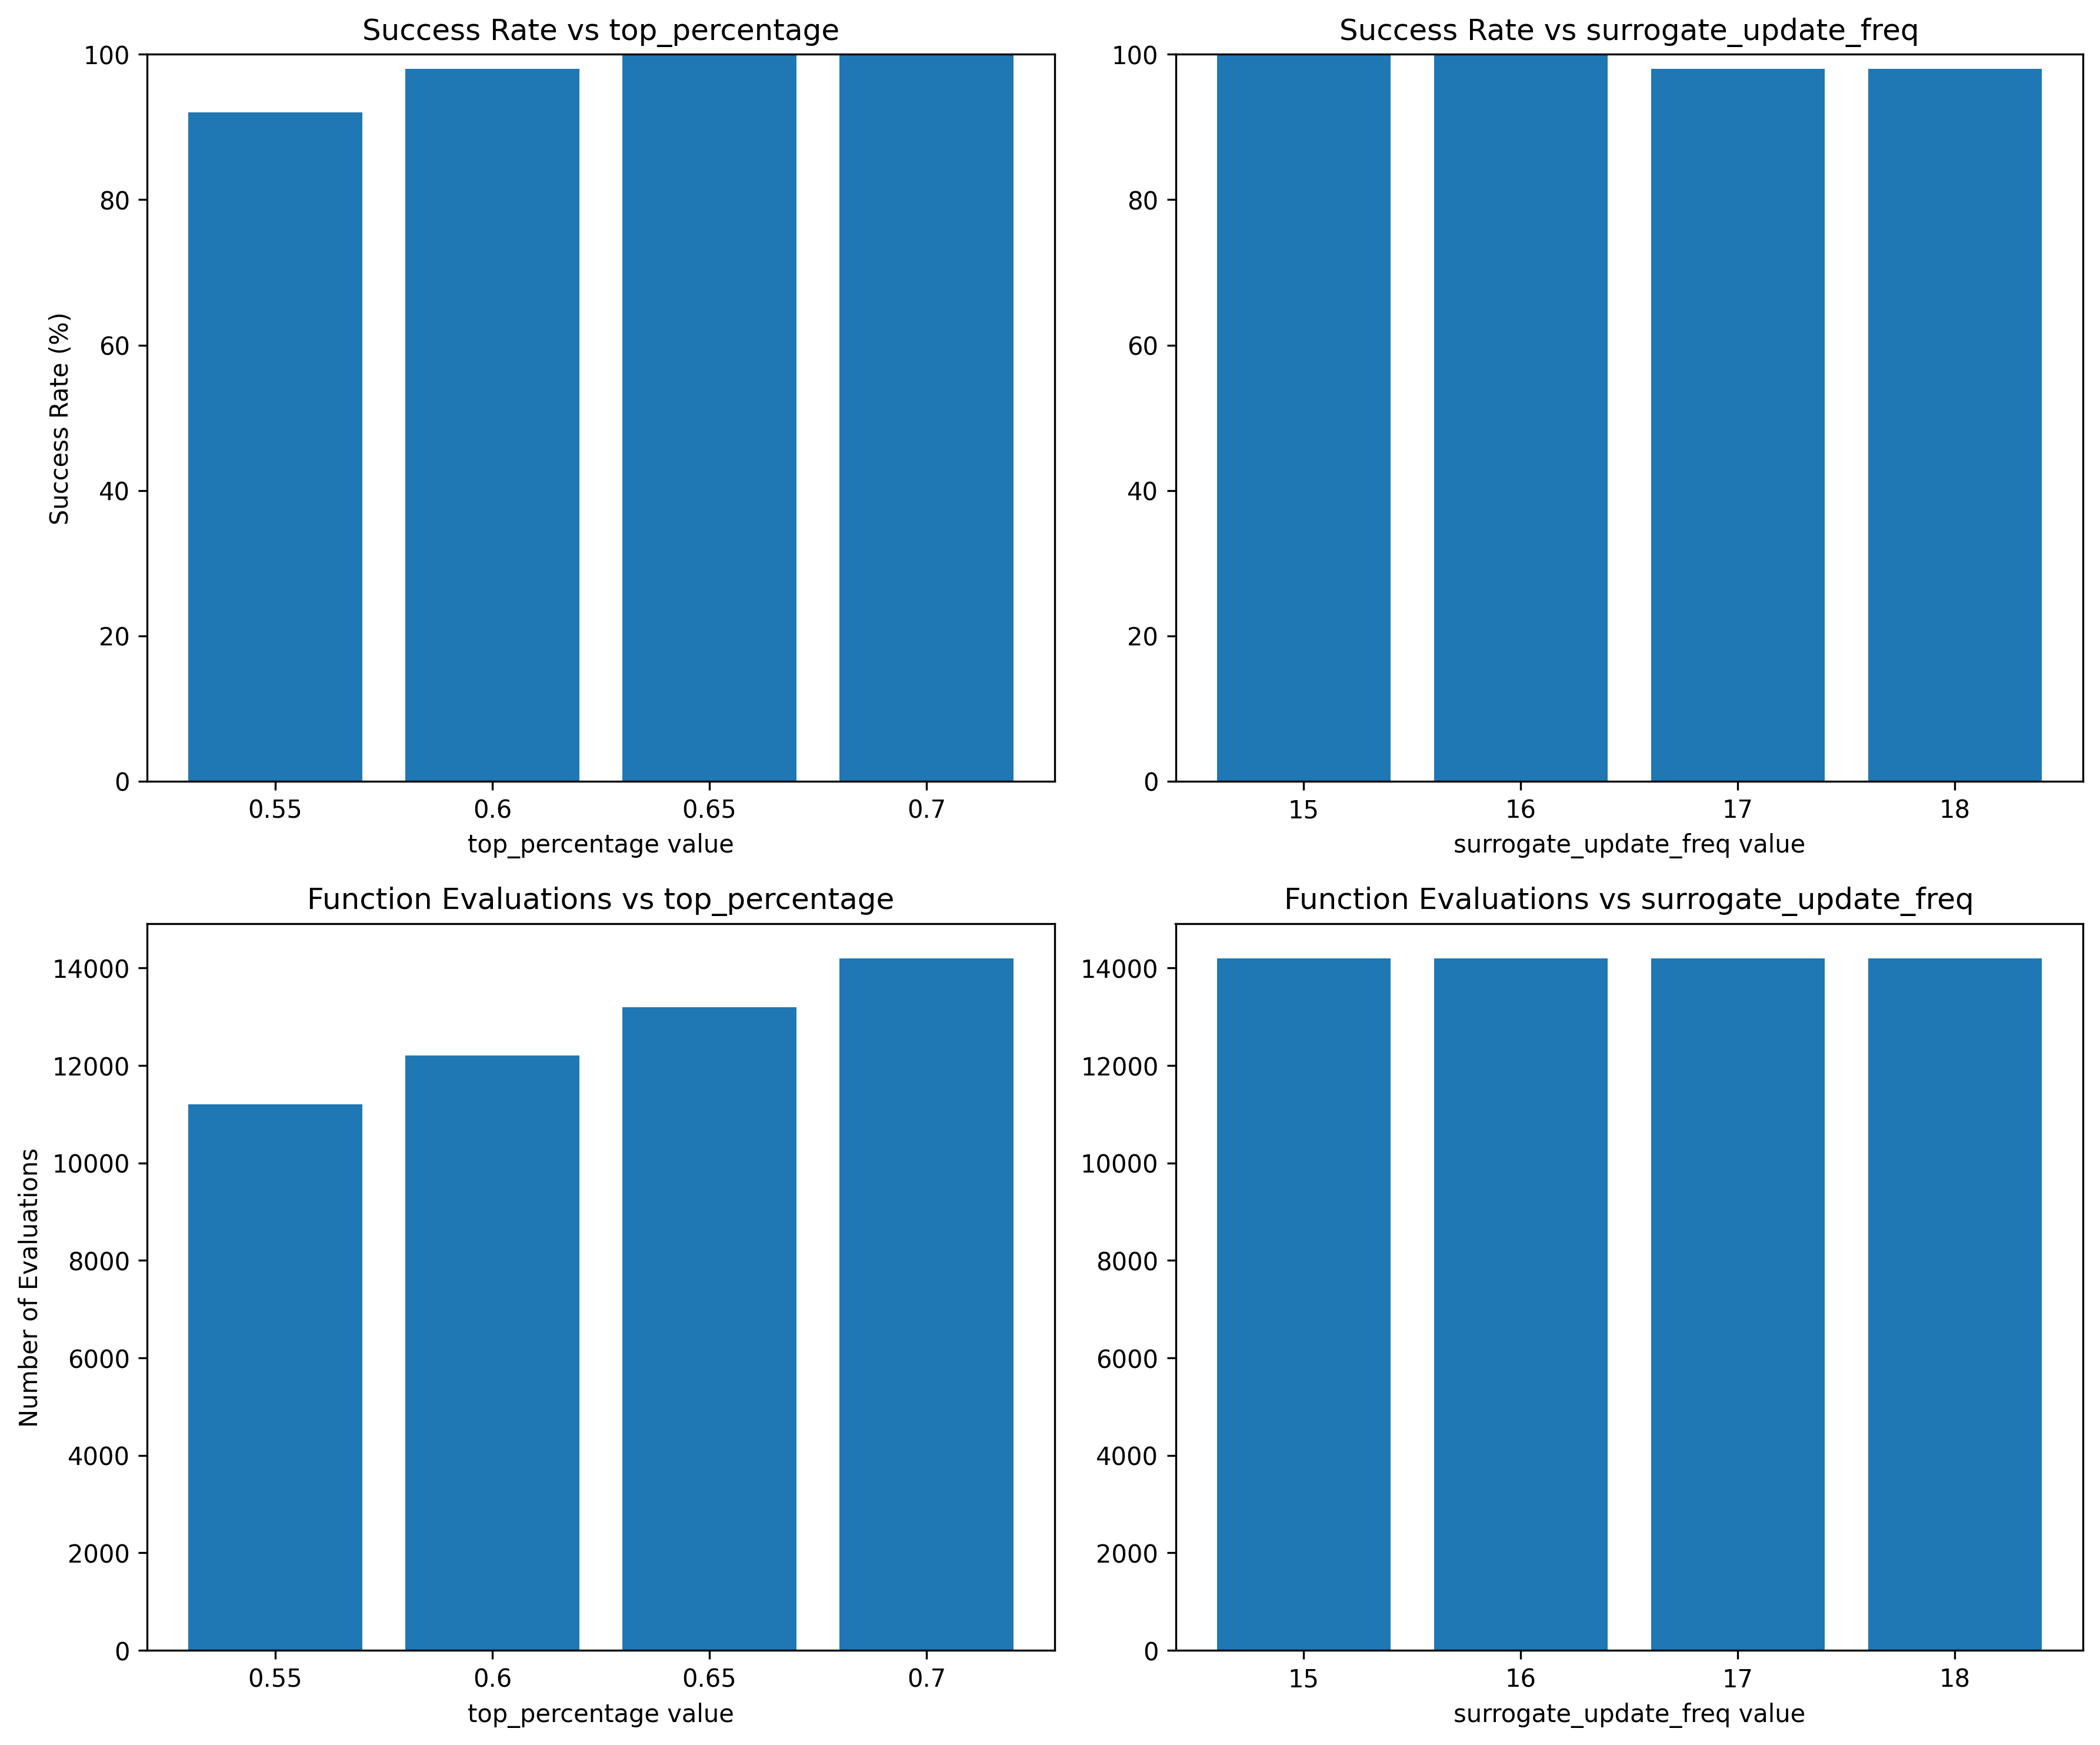
\includegraphics[width=\textwidth]{surrogate_de_parameter_tuning_results3.png}
    \caption{Wpływ procentu najlepszych rozwiązań, które są ewaluowane oraz częstotliwości uczenia modelu na skuteczność działania algorytmu dla następujących wartości domyślnych: procent najlepszych rozwiązań = 0.7, częstotliwość uczenia = 15}
    \label{fig:surogate_de_parameter_results3}
\end{figure}


\subsection{Zmiany w sekcji: model zastępczy}

Dodano informacje o historii punktów zewaluowanych.

Historia zewaluowanych punktów nie ma ograniczonego rozmiaru, a dodane do niej punkty nie są usuwane. Zapewnia to pełną informację o przestrzeniu przeszukiwań.
\end{document}